\documentclass{beamer}
\usepackage{amsmath, xparse}


\usetheme{Warsaw}


\iftrue

\setbeamercolor{normal text}{fg=white,bg=black!90}
\setbeamercolor{structure}{fg=white}

\setbeamercolor{alerted text}{fg=red!85!black}

\setbeamercolor{item projected}{use=item,fg=black,bg=item.fg!35}

\setbeamercolor*{palette primary}{use=structure,fg=structure.fg}
\setbeamercolor*{palette secondary}{use=structure,fg=structure.fg!95!black}
\setbeamercolor*{palette tertiary}{use=structure,fg=structure.fg!90!black}
\setbeamercolor*{palette quaternary}{use=structure,fg=structure.fg!95!black,bg=black!80}

\setbeamercolor*{framesubtitle}{fg=white}

\setbeamercolor*{block title}{parent=structure,bg=black!60}
\setbeamercolor*{block body}{fg=black,bg=black!10}
\setbeamercolor*{block title alerted}{parent=alerted text,bg=black!15}
\setbeamercolor*{block title example}{parent=example text,bg=black!15}

\fi


\begin{document}

{
    \usebackgroundtemplate
    {
        \vbox to \paperheight{\vfil\hbox to \paperwidth{\hfil

        {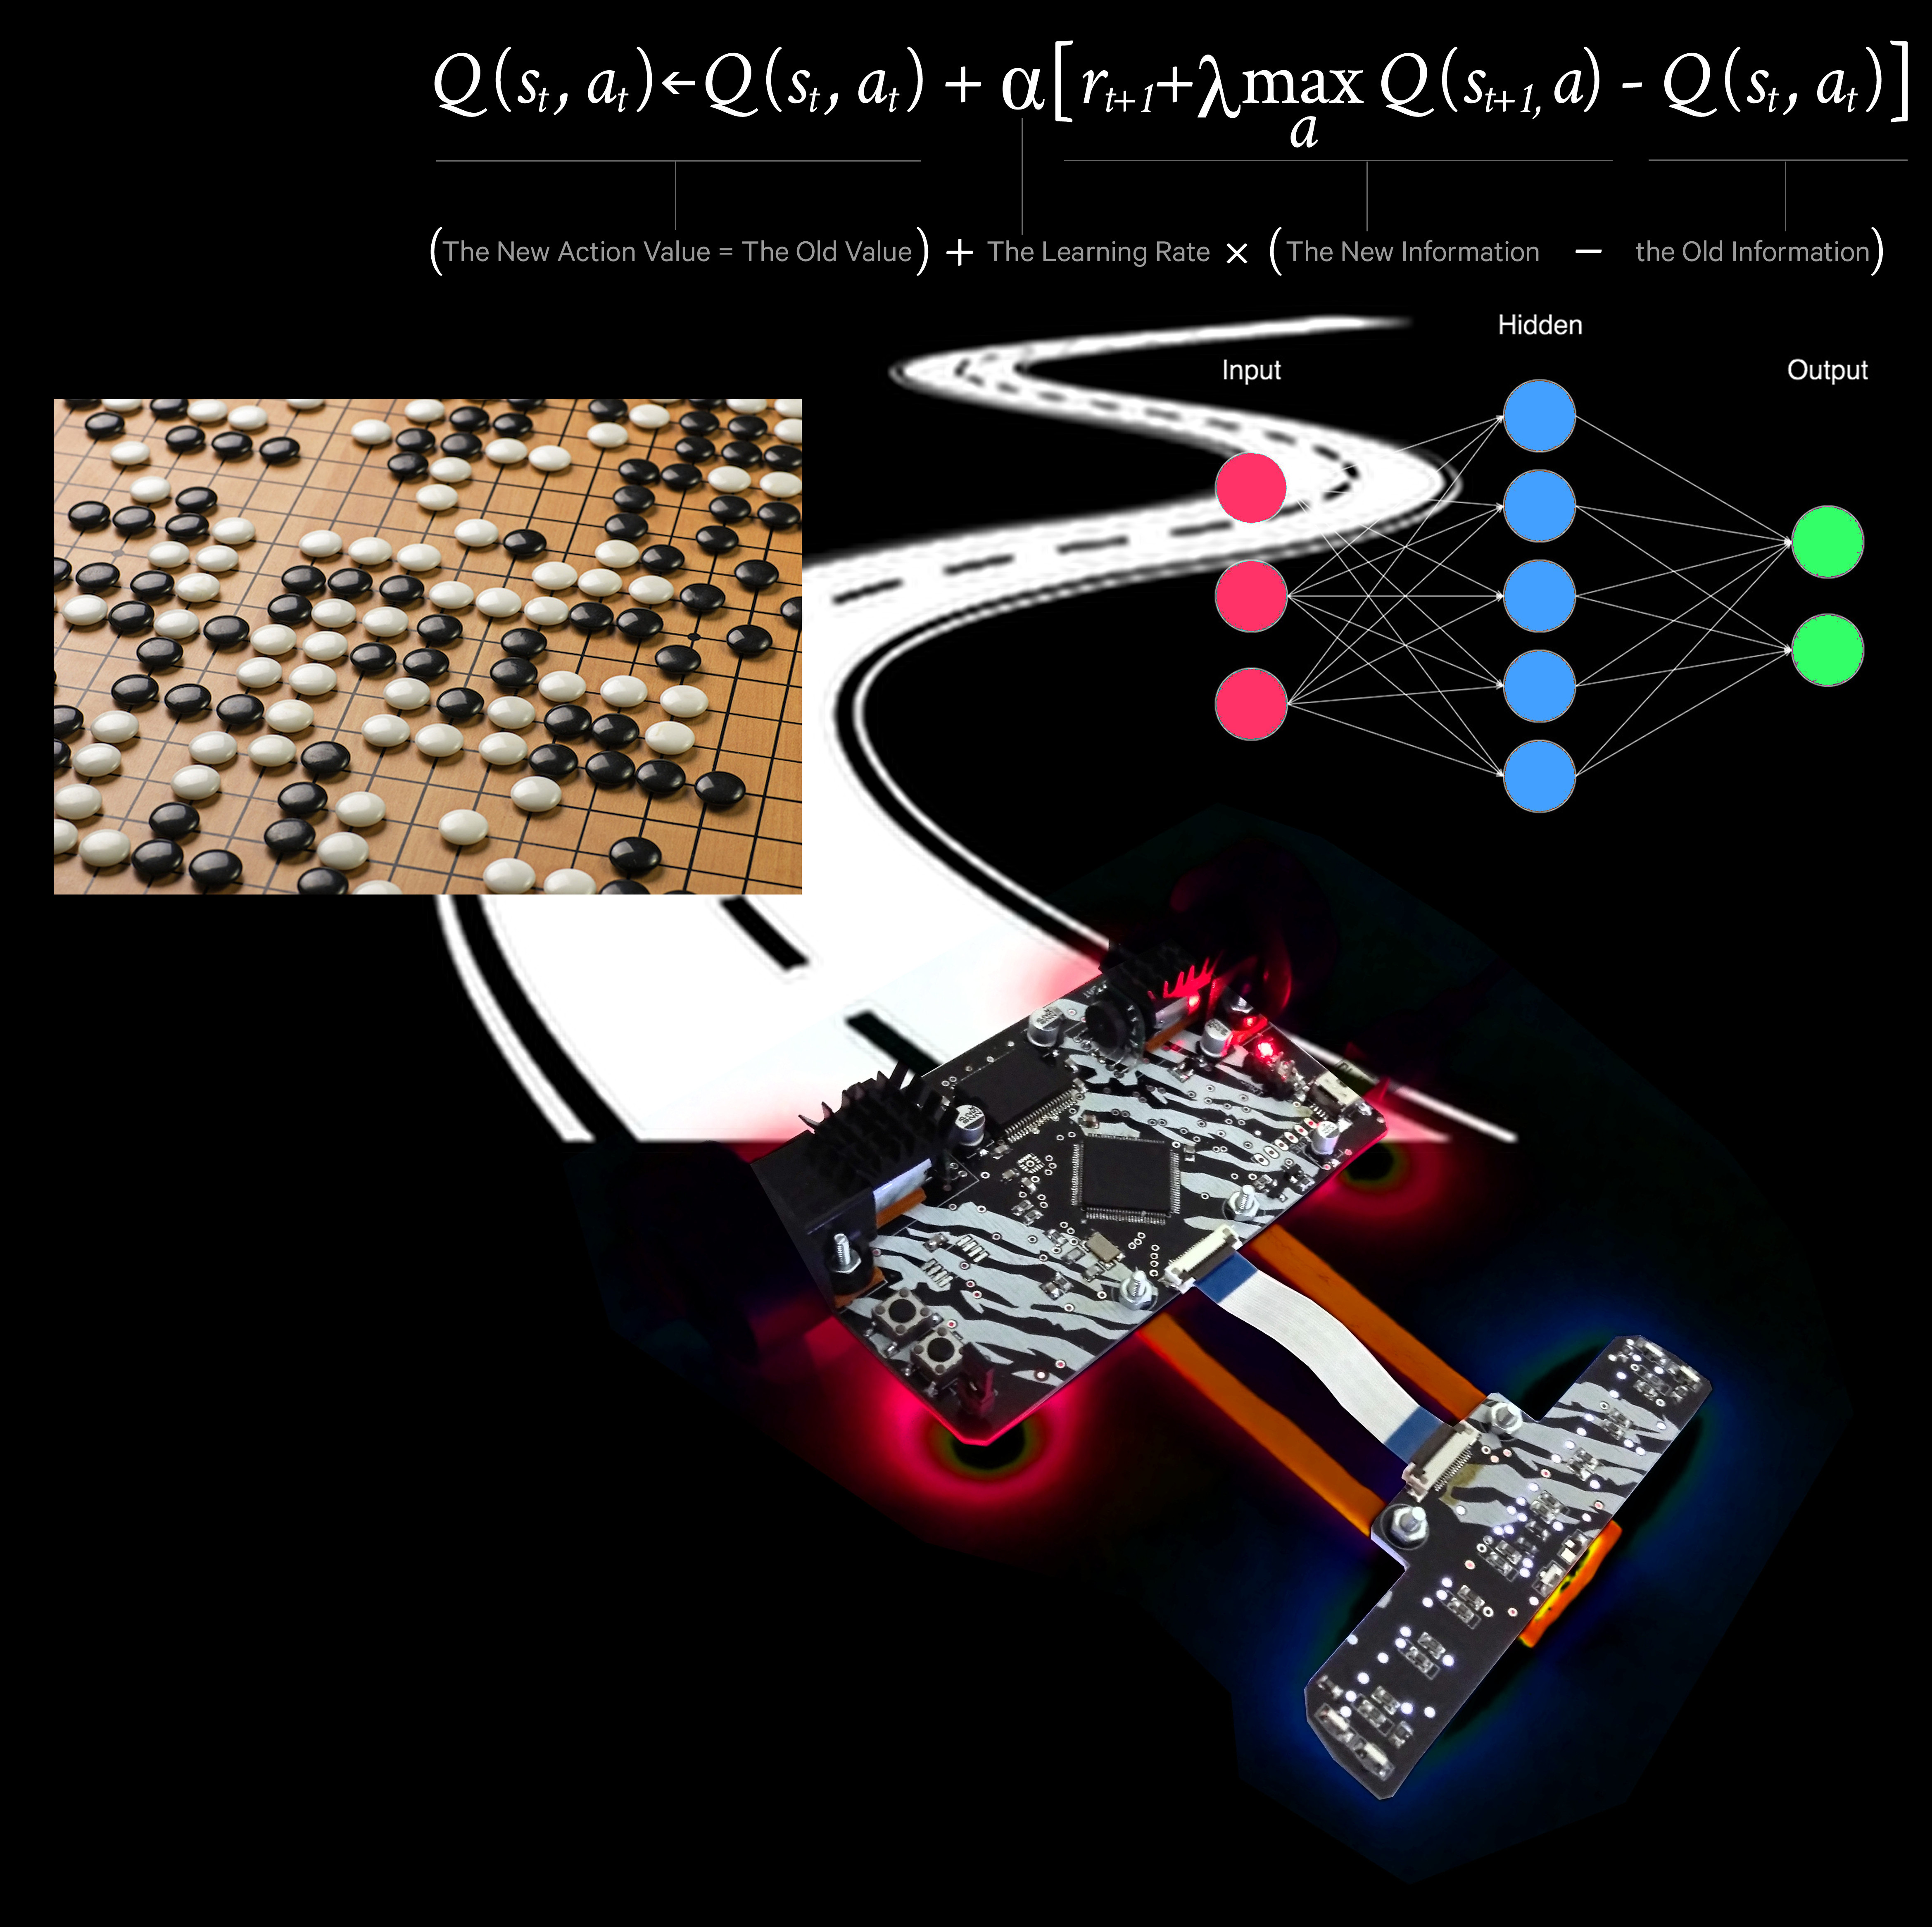
\includegraphics[width=5.05in]{../images/generic/rl_square.jpg}}

        \hfil}\vfil}
    }

    \begin{frame}
     \centering
     \colorbox{black}
     {
        \begin{minipage}{8cm}
           {\LARGE \color{white}{\textbf { model predictive control}} \\}
           {\LARGE \color{white}{\textbf { Michal CHOVANEC, PhD.}} \\}
       \end{minipage}
     }

    \end{frame}
}



\begin{frame}
  
  \frametitle{\textbf { MPC - applications }}

  \begin{columns}

    \begin{column}{0.5\textwidth}
      \centering{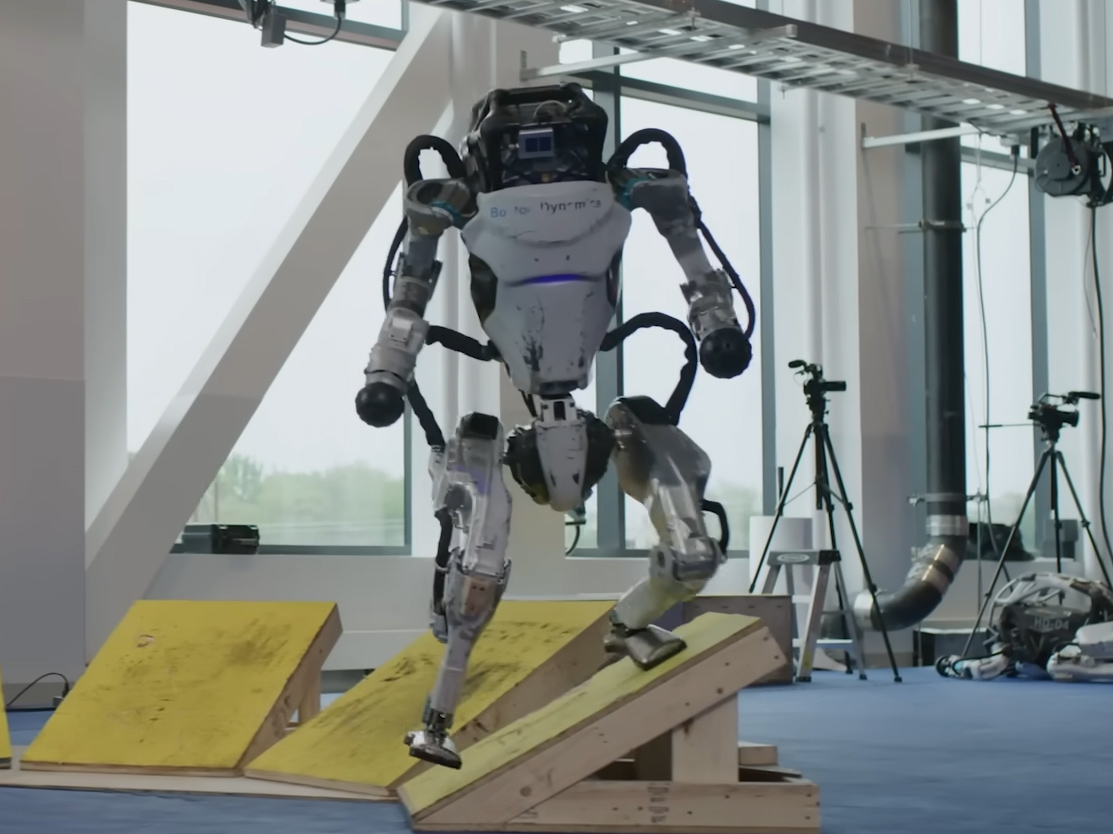
\includegraphics[scale=0.1]{../images/generic/boston_dynamics.jpeg}} \\
      \centering{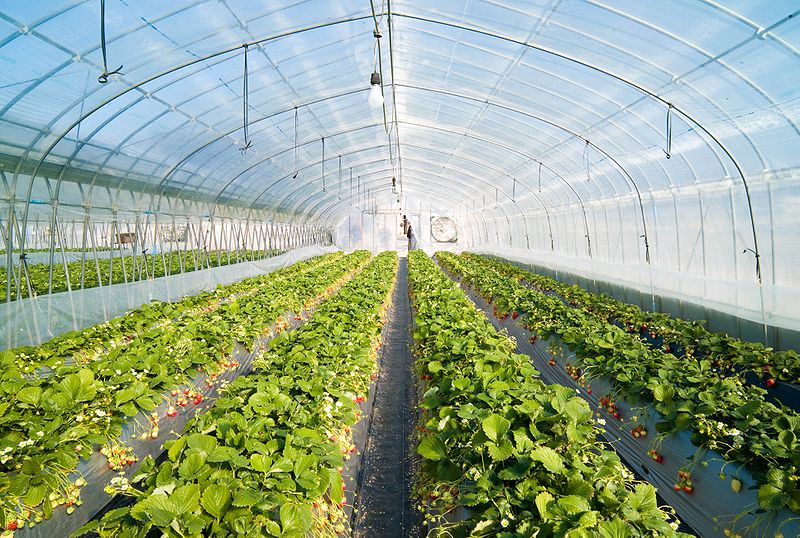
\includegraphics[scale=0.4]{../images/generic/green_house.jpeg}}
    \end{column}

    \begin{column}{0.5\textwidth}

      \centering{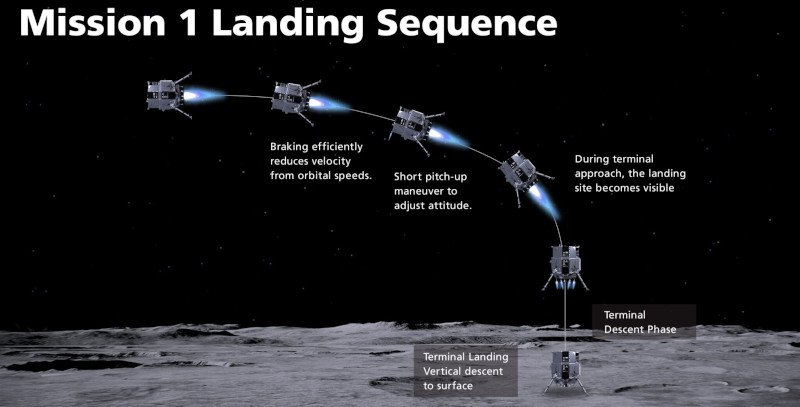
\includegraphics[scale=0.2]{../images/generic/hakuto.jpeg}} \\
      \centering{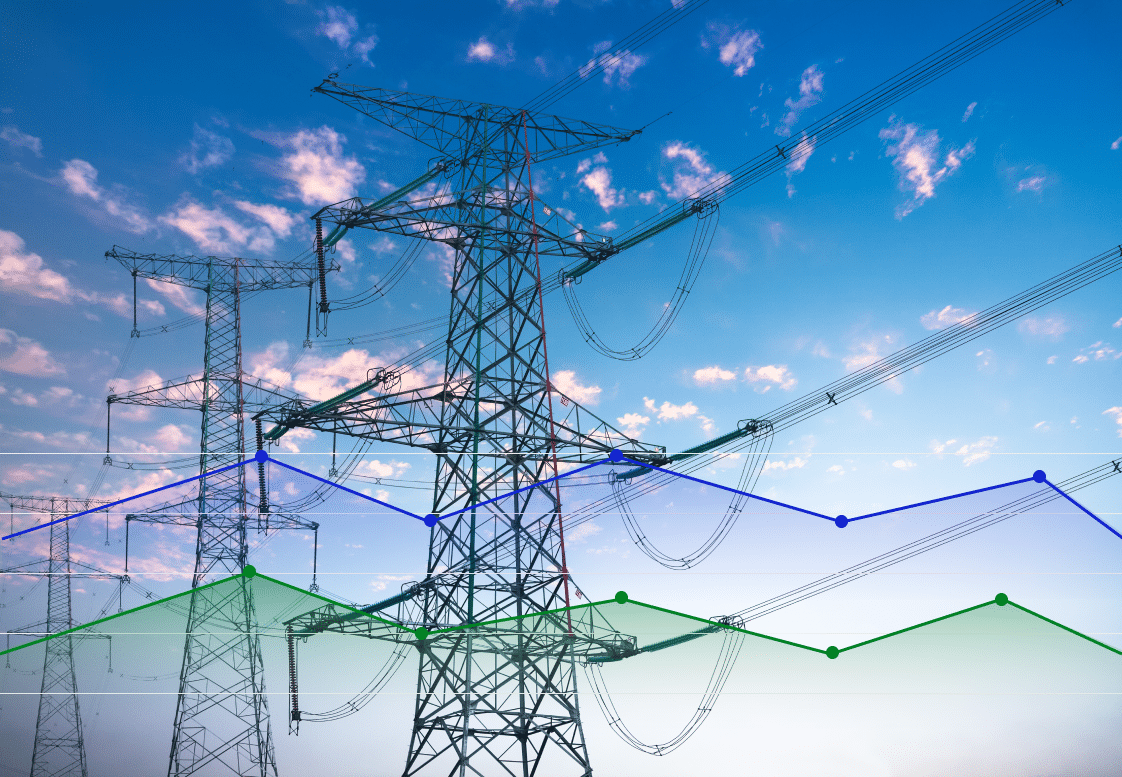
\includegraphics[scale=0.1]{../images/generic/smart_grid.png}}
      
    \end{column}

  \end{columns}


\end{frame}









\begin{frame}
  
  \frametitle{\textbf { MPC - overview }}
  \centering{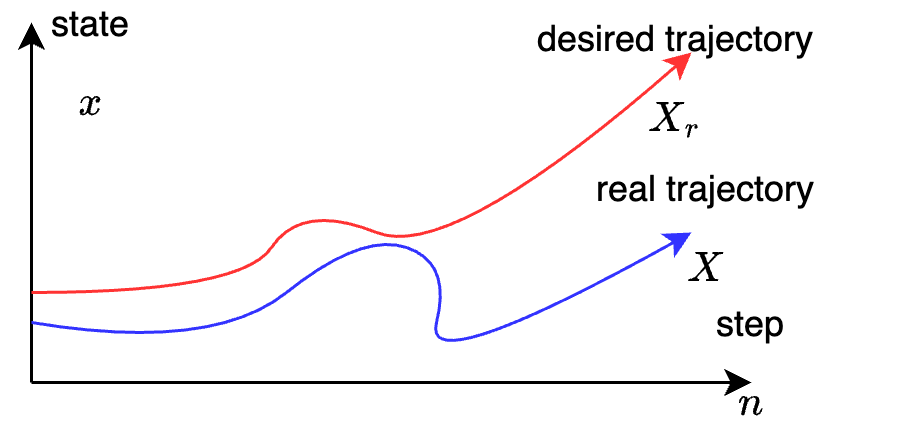
\includegraphics[scale=1.0]{../diagrams/control/control-mpc_overview_0.png}}

\end{frame}

\begin{frame}
  
  \frametitle{\textbf { MPC - overview }}
  \centering{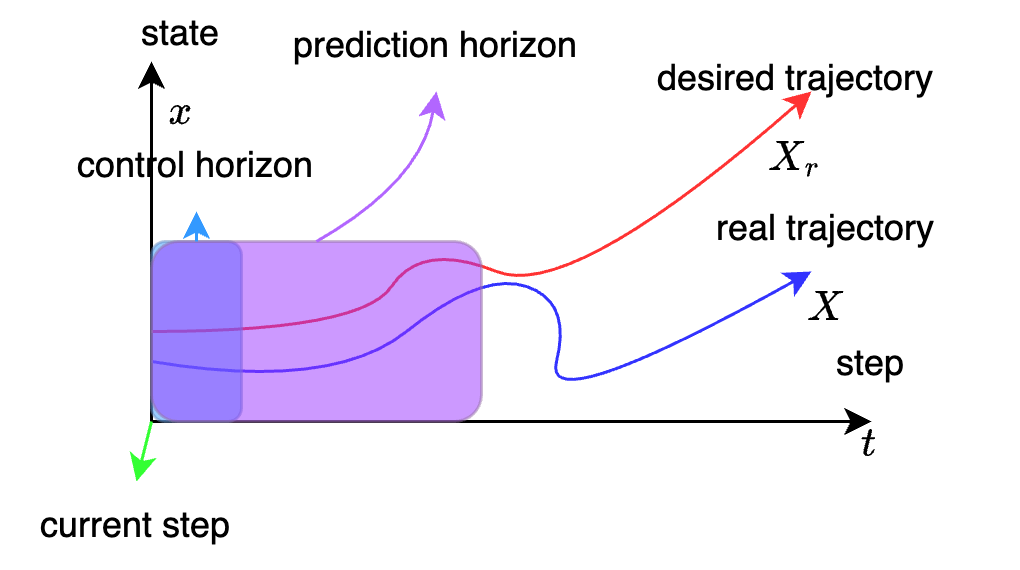
\includegraphics[scale=0.9]{../diagrams/control/control-mpc_overview_1.png}}
  
 
  \begin{columns}

    \begin{column}{0.5\textwidth}
      state vector, \\ e.g. (position, velocity, angle, angular rate)
      \begin{align*}
        x &=
        \begin{bmatrix}
          x_0 \\
          x_1 \\
          ..  \\
          x_{n-1}  
        \end{bmatrix}
      \end{align*}
    \end{column}

    \begin{column}{0.5\textwidth}
      control variable, \\ e.g. (left speed, right speed)
      \begin{align*}
        u &=
        \begin{bmatrix}
          u_0 \\
          u_1 \\
          ..  \\
          u_{m-1}  
        \end{bmatrix}
      \end{align*}
    \end{column}

  \end{columns}

\end{frame}






\begin{frame}
  
  \frametitle{\textbf { robot trajectory tracking example}}
  \centering{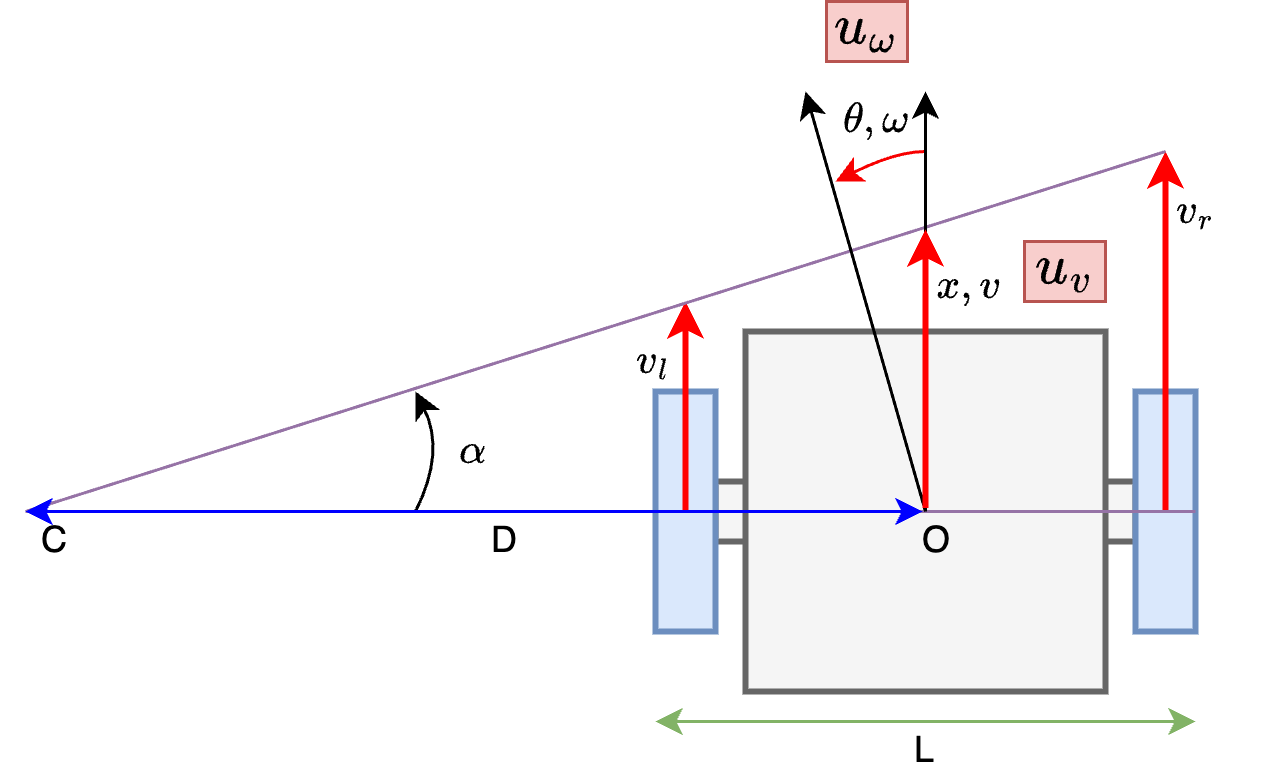
\includegraphics[scale=1.0]{../diagrams/robot/robot-differential_drive.png}}

\end{frame}


\begin{frame}
  
  \frametitle{\textbf { robot trajectory tracking example}}
 
  \begin{columns}

    \begin{column}{0.5\textwidth}
      \centering{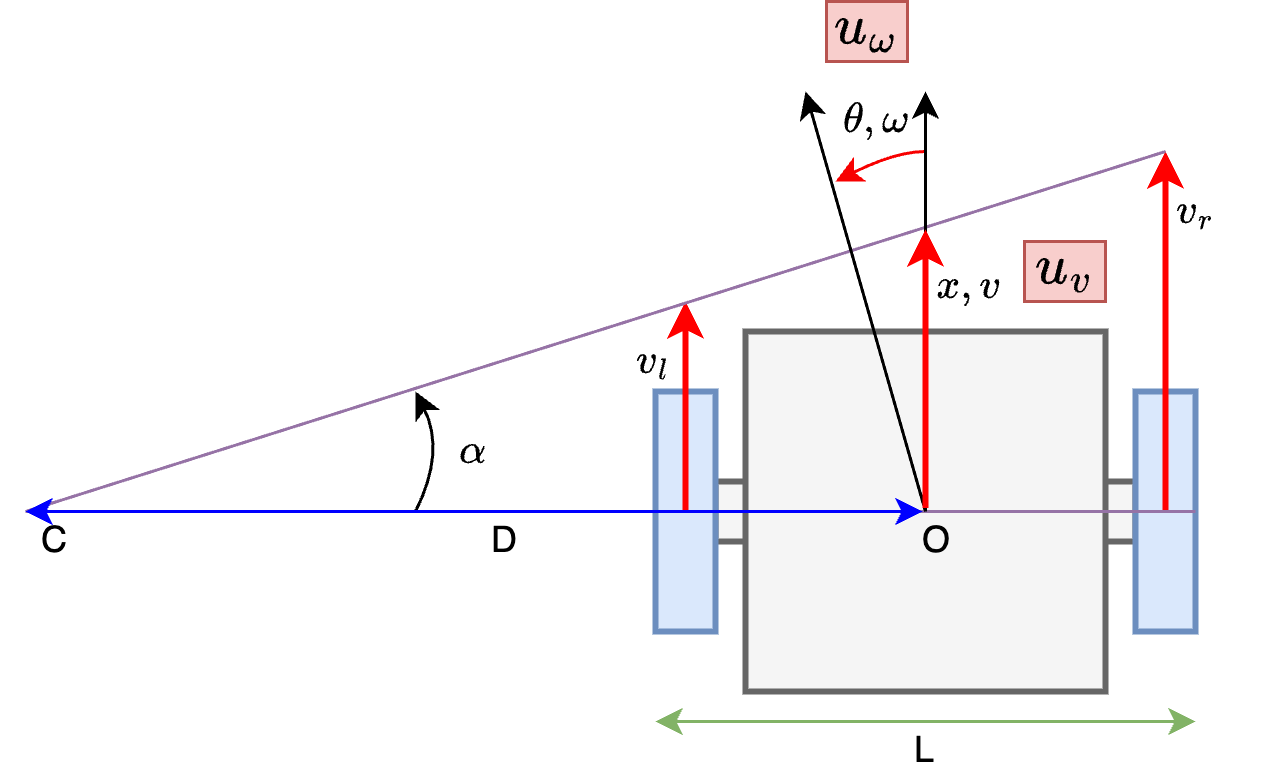
\includegraphics[scale=0.5]{../diagrams/robot/robot-differential_drive.png}}
    \end{column}

    \begin{column}{0.5\textwidth}
      \begin{itemize}
        \item state
          \begin{align*}
            x &=
            \begin{bmatrix}
              v \\
              d \\
              \omega \\
              \theta
            \end{bmatrix}
          \end{align*}


        \item control variable
          \begin{align*}
            _\Delta u &=
            \begin{bmatrix}
              _\Delta u_v \\
              _\Delta u_{\omega}
            \end{bmatrix}
          \end{align*}

          \begin{align*}
            u(n) &= u(n-1) +{_\Delta}u(n)
          \end{align*}

      \end{itemize}
    \end{column}

  \end{columns}

\end{frame}





\begin{frame}
\frametitle{\textbf { state space model (continuos)}}

  \begin{align*}
    dx &= Ax + Bu
  \end{align*}
  
  \begin{columns}

    \begin{column}{0.5\textwidth}

      \begin{align*}
        A =
        \begin{pmatrix}
          -\frac{1}{\tau_{forward}} & 0 & 0 & 0 \\
          1 & 0 & 0 & 0 \\
          0 & 0 & -\frac{1}{\tau_{turn}} & 0 \\
          0 & 0 & 1 & 0 
        \end{pmatrix}
      \end{align*}
    
    \end{column}


    \begin{column}{0.5\textwidth}

      \begin{align*}
        B =
        \begin{pmatrix}
          -\frac{k_{forward}}{\tau_{forward}} & 0 \\
          0 & 0 \\
          0 & -\frac{k_{turn}}{\tau_{turn}} \\
          0 & 0
        \end{pmatrix}
      \end{align*}

    \end{column}


  \end{columns}

  \begin{itemize}
    \item 4 poles : double in $0$, $-\frac{1}{\tau_{forward}}$ and $-\frac{1}{\tau_{turn}}$
    \item 2 control inputs : forward velocity and turning velocity
    \item constrains for kick avoid (jerk) : ${_\Delta}u_{min} < {_\Delta}u < {_\Delta}u_{max}$
    \item constrains for motor limits : $u_{min} < u < u_{max}$
  \end{itemize}

\end{frame}



\begin{frame}
  
  \frametitle{\textbf { MPC - overview }}
  \centering{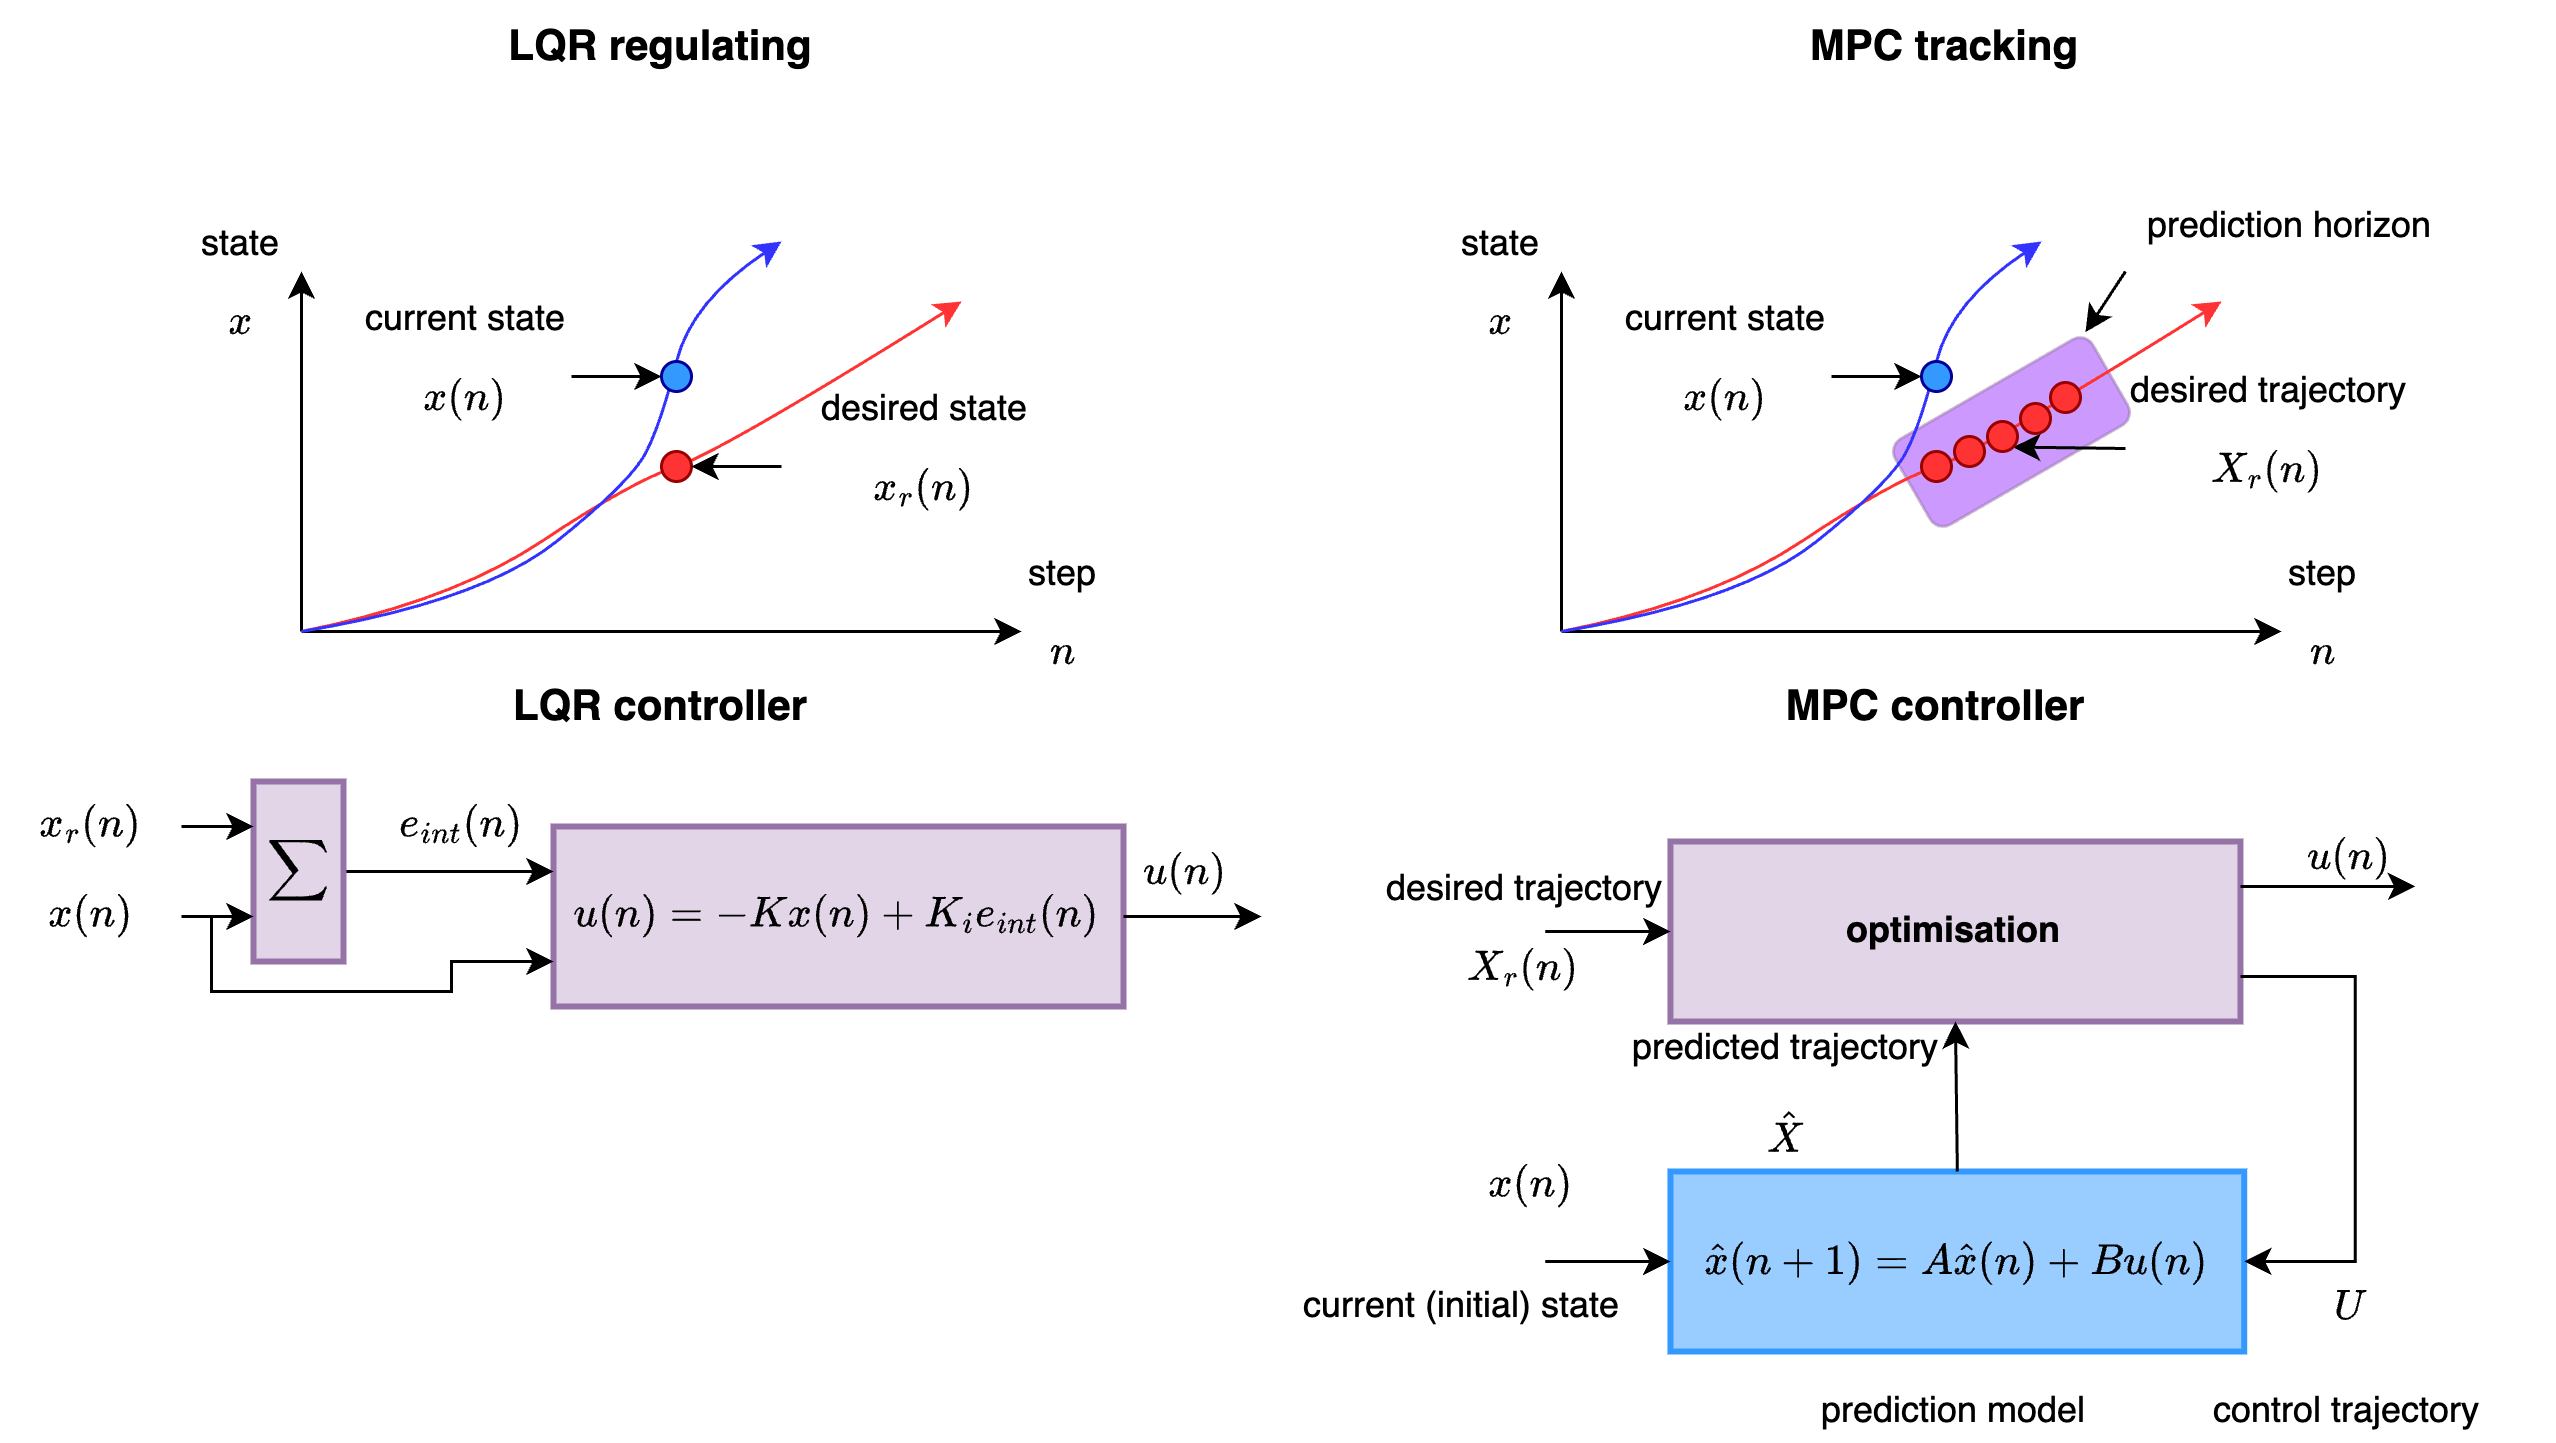
\includegraphics[scale=0.55]{../diagrams/control/control-robot_tracking.png}}

\end{frame}



\begin{frame}
  
  \frametitle{\textbf { MPC - overview }}
  \centering{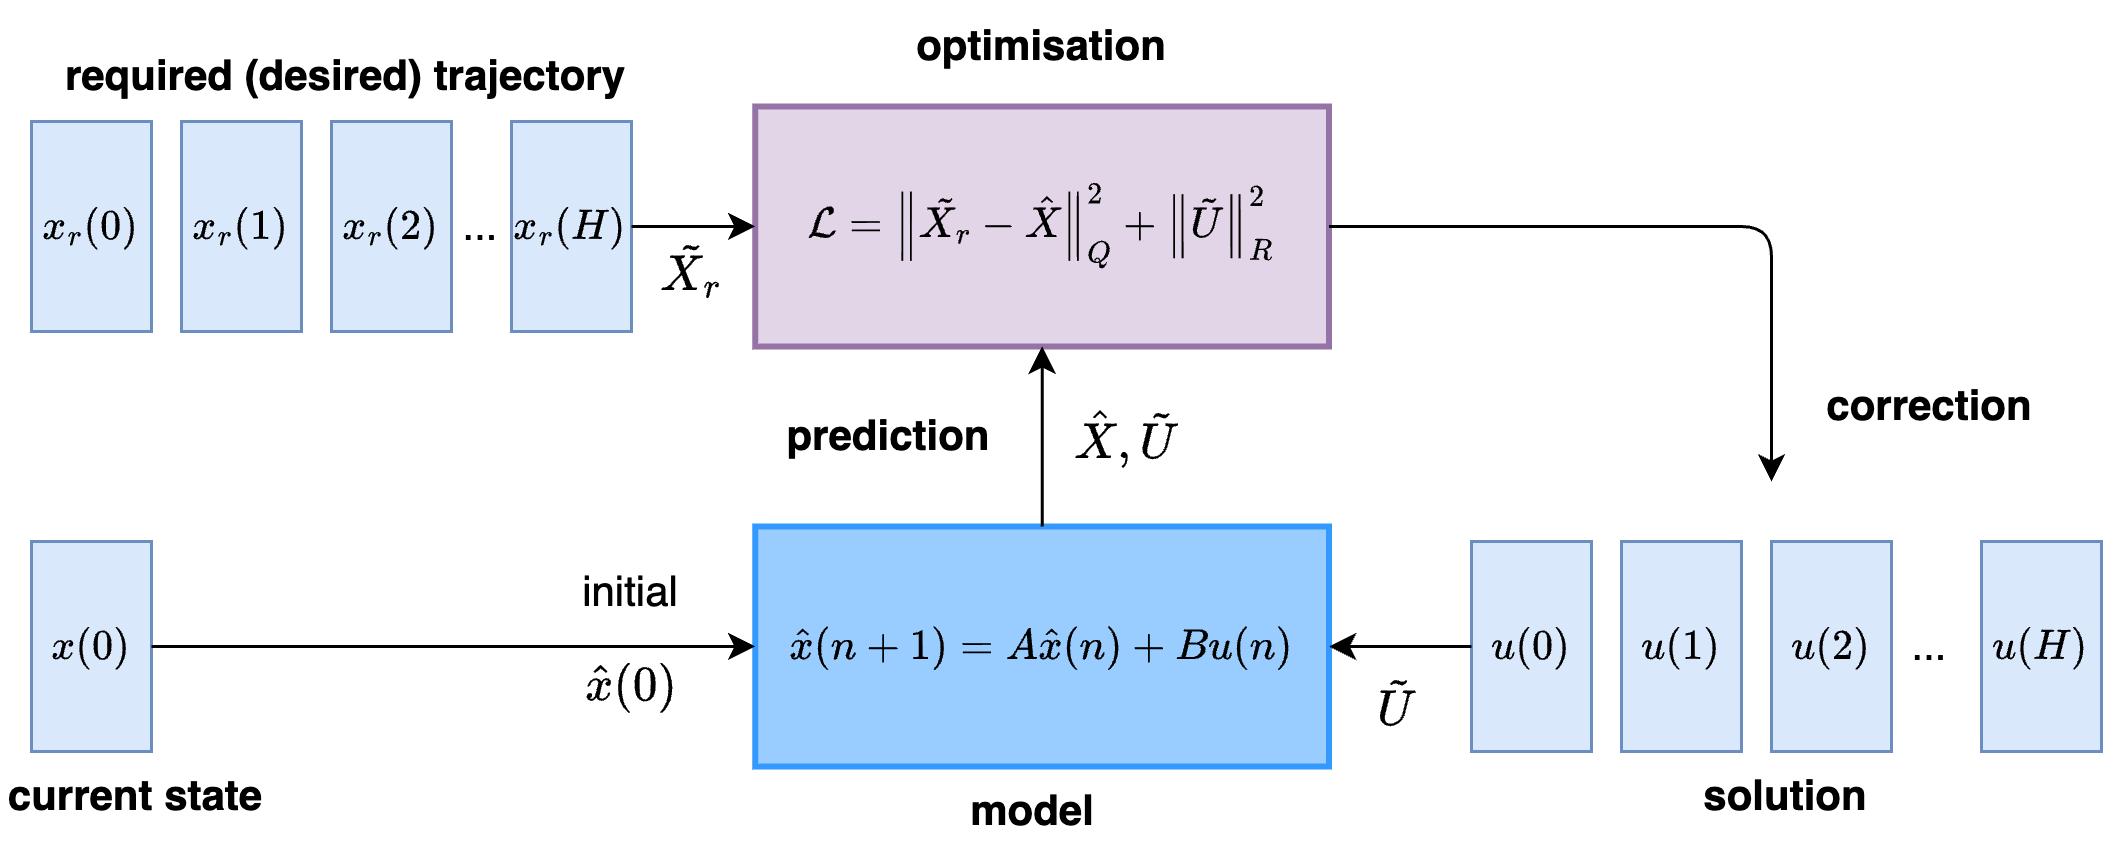
\includegraphics[scale=0.65]{../diagrams/control/control-mpc_overview_2.png}}

\end{frame}






\begin{frame}
  
  \frametitle{\bf quadratic problem formulation}

  \centering{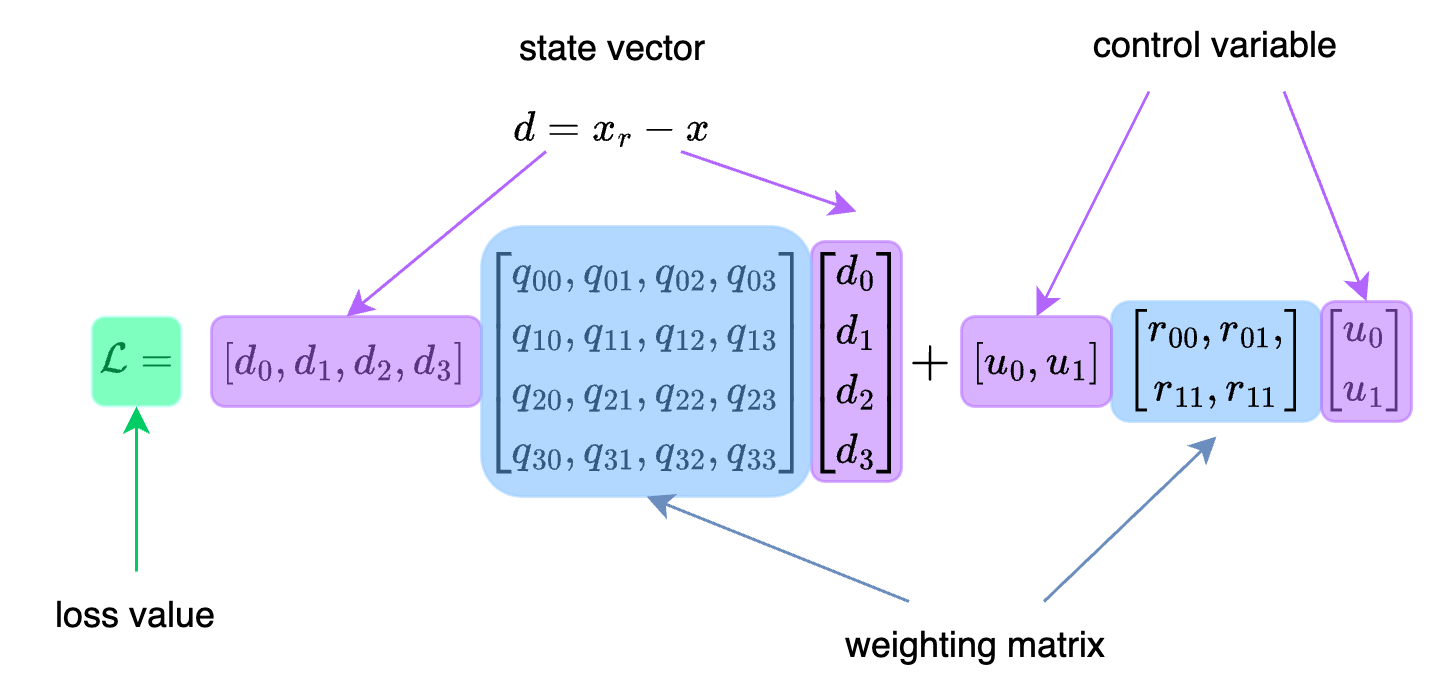
\includegraphics[scale=0.8]{../diagrams/control/control-q_loss.png}}
  
\end{frame}




\begin{frame}
  
  \frametitle{\bf quadratic problem formulation}

  loss (cost) function is quadratic, with weighting terms $Q$ and $R$,

  \begin{align*}
    \mathcal{L} = \sum_{h=0}^{H-1} \big((x_r(h) - x(h))^T Q (x_r(h) - x(h))\big) +_{\Delta}u^T(h)R_{\Delta}u(h), \\
    u(n) = u(n-1)+_{\Delta}u(n), \\
    \text{s.t.} \quad x(n+1) = Ax(n) + Bu(n).
  \end{align*}

  where : 
  \begin{itemize}
    \item $H$ is prediction horizon steps
    \item $A$ is matrix, $n \times n$
    \item $B$ is matrix, $n \times m$
    \item $Q$ is matrix, $n \times n$
    \item $R$ is matrix, $m \times m$
    \item $_{\Delta}u$ is controller output
    \item where $n$ is system orders, and $m$ system inputs count
  \end{itemize}

  
\end{frame}


\begin{frame}
  
  \frametitle{\bf unrolling sequence}
  rewrite into form where initial conditions {\bf depends only} on $x(n)$ and $u(n-1)$ 
  \begin{align*}
    x(n+1)&= Ax(n) + Bu(n) \\
          &= Ax(n) + B(u(n-1) + _\Delta u(n)) \\
    x(n+2)&= Ax(n+1) + B(u(n) + _\Delta u(n+1)) \\
          &= A^2x(n) + (AB + B)u(n-1) + (AB+B)_\Delta u(n) + B_\Delta u(u) \\
    x(n+3)&= Ax(n+2) + B(u(n+1) + _\Delta u(n+2)) \\
          &= A^3x(n) + (A^2 + AB + B)u(n-1) \\
          & + (A^2B + AB + B)_\Delta u(n) \\
          & + (AB + B)_\Delta u(n+1) + B_\Delta u(n+2) \\
    ... 
  \end{align*}  

  
\end{frame}






\begin{frame}
  
  \frametitle{\bf matrix formulation}
  rewrite into matrix form
  \begin{align*}
    \begin{bmatrix}
      x(n+1) \\
      x(n+2) \\
      \dots \\
      x(n+H)
    \end{bmatrix} &= 
    \begin{bmatrix}
      A^1 \\
      A^2 \\
      \dots \\
      A^H
    \end{bmatrix} x(n) +
    \begin{bmatrix}
      B \\
      AB \\
      \dots \\
      \sum_{i=0}^{H-1} A^iB
    \end{bmatrix} u(n-1) + \\
    &+
    \begin{bmatrix}
      B  & 0 & \dots & 0 \\
      AB + B & B & \dots & 0 \\
      \dots & \dots & \dots & \dots \\
      \sum_{i=0}^{H-1}A^iB & \sum_{i=0}^{H-2}A^iB & \dots & B
    \end{bmatrix}
    \begin{bmatrix}
      _\Delta u(n) \\
      \dots \\
      _\Delta u(n + H - 1) \\
    \end{bmatrix} 
  \end{align*}

  in compaxt form

  \begin{align*}
    \tilde{X} &= \Psi x(n) + \Omega u(n-1) + \Theta \tilde{_\Delta U}
  \end{align*}


\end{frame}




\begin{frame}
  
  \frametitle{\bf matrix formulation}

  \centering{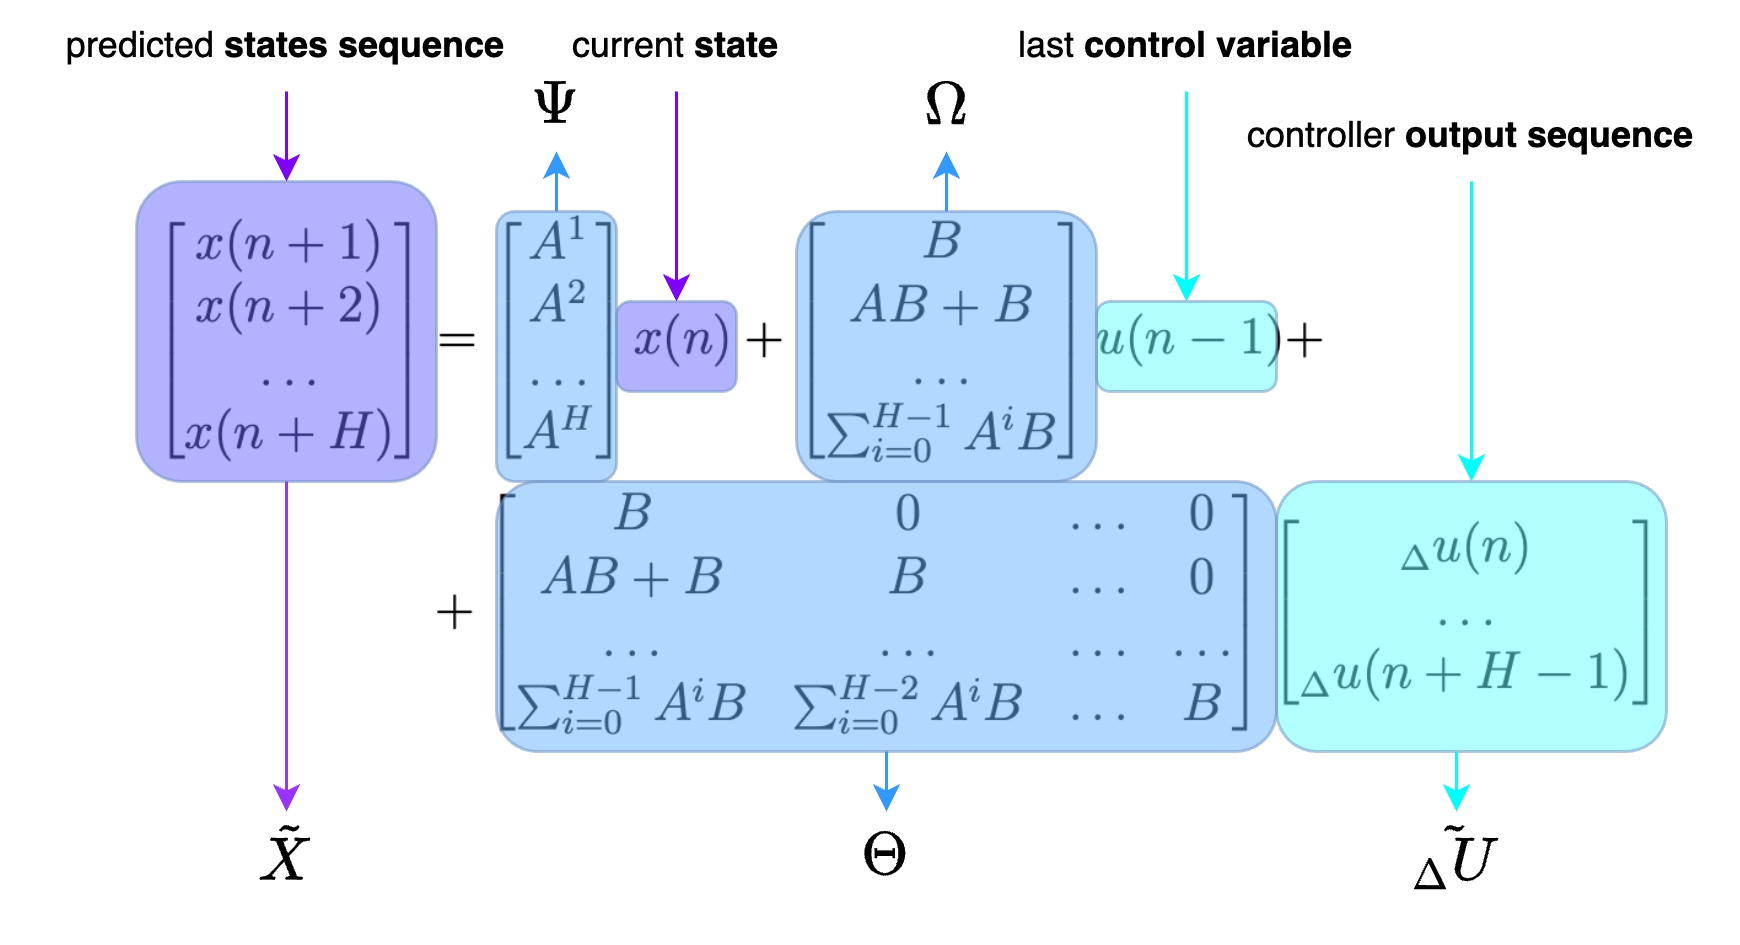
\includegraphics[scale=0.65]{../diagrams/control/control-mpc_exp_0.png}}

  \begin{align*}
    \tilde{X} &= \Psi x(n) + \Omega u(n-1) + \Theta \tilde{_\Delta U}
  \end{align*}
\end{frame}




\begin{frame}
  
  \frametitle{\bf n-th step input to output projection}

  \centering{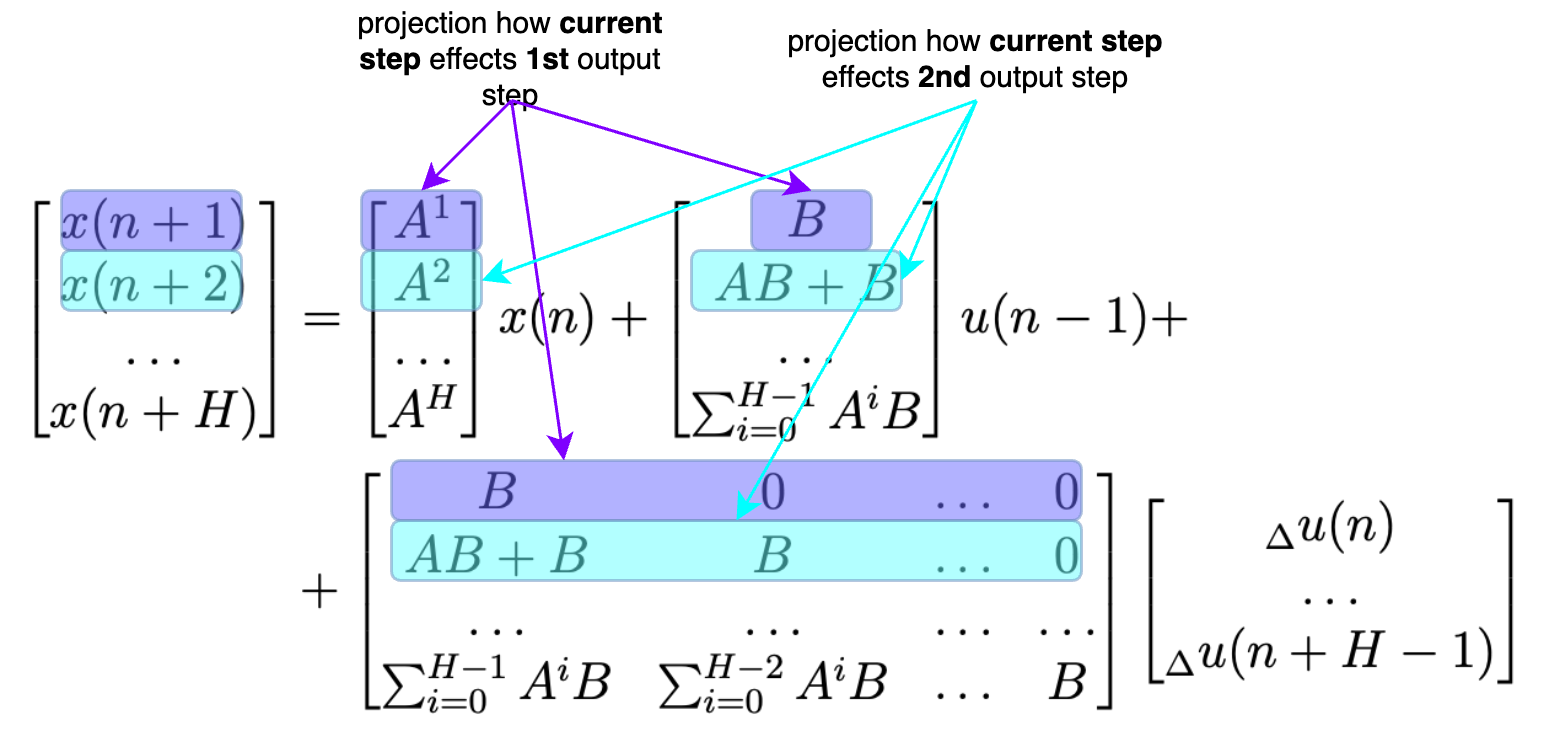
\includegraphics[scale=0.75]{../diagrams/control/control-mpc_exp_1.png}}

\end{frame}



\begin{frame}
  
  \frametitle{\bf projection of controll $_\Delta u(n)$ to output sequence}

  \centering{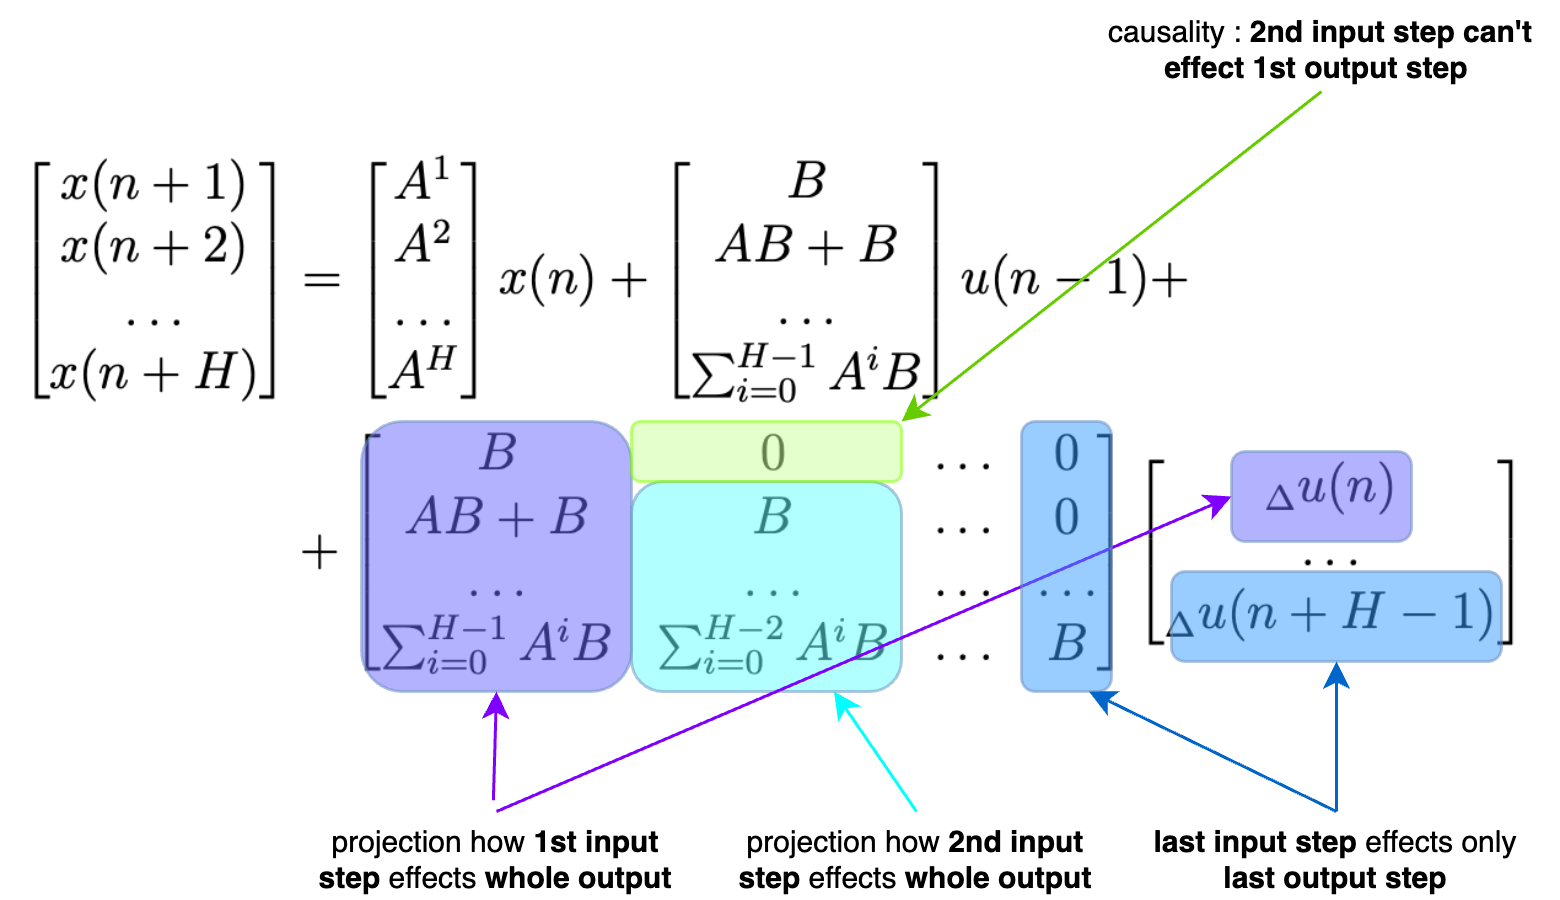
\includegraphics[scale=0.75]{../diagrams/control/control-mpc_exp_2.png}}

\end{frame}



\begin{frame}
  
  \frametitle{\bf $Q$ and $R$ augmentation}

  \centering{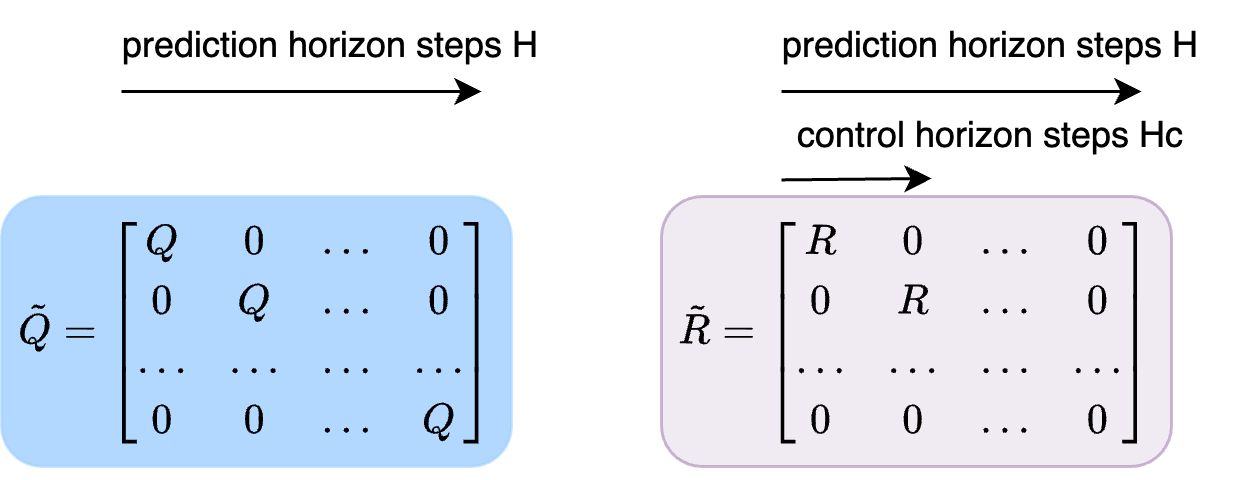
\includegraphics[scale=0.75]{../diagrams/control/control-q_aug.png}}

\end{frame}



\begin{frame}
  
  \frametitle{\bf put into quadratic loss (cost) function}

  \begin{align*}
    \mathcal{L} &= \tilde{_\Delta U}^T \tilde{R} \tilde{_\Delta U} 
                + (\tilde{X_r} - \tilde{X})^T \tilde{Q} (\tilde{X_r} - \tilde{X}) \\
  \end{align*}

  after substitution
  \begin{align*}
    S = \tilde{X_r} - \Psi\tilde{X} - \Omega u(n-1)
  \end{align*}

  we obtain
  \begin{align*}
    \mathcal{L} &= \tilde{_\Delta U}^T \tilde{R} \tilde{_\Delta U} + (S -  \Theta \tilde{_\Delta U} )^T \tilde{Q} (S -  \Theta \tilde{_\Delta U} ) \\
                &= \tilde{_\Delta U}^T \tilde{R} \tilde{_\Delta U} 
                + S^T\tilde{Q}S - S^T \tilde{Q} \Theta \tilde{_\Delta U} 
                - \tilde{_\Delta U}^T \Theta^T\tilde{Q}S + \tilde{_\Delta U}^T\Theta^T\tilde{Q}\Theta\tilde{_\Delta U}
  \end{align*}

\end{frame}



\begin{frame}
  
  \frametitle{\bf finding minima}

  find derivative with respect to $\tilde{_\Delta U}$ 

  \begin{align*}  
    \frac{\partial \mathcal{L}}{\partial {\tilde{_\Delta U}}} & : \\
    \frac{\partial {\tilde{_\Delta U}^T \tilde{R} \tilde{_\Delta U} } }{\partial {\tilde{_\Delta U}}} & = 2\tilde{R}\tilde{_\Delta U} \\
    \frac{\partial {S^T\tilde{Q}S}}{\partial {\tilde{_\Delta U}}} & = 0 \\
    \frac{\partial {- S^T \tilde{Q} \Theta \tilde{_\Delta U} }}{\partial {\tilde{_\Delta U}}} & = -\Theta^T\tilde{Q}S \\
    \frac{\partial {- \tilde{_\Delta U}^T \Theta^T\tilde{Q}S}}{\partial {\tilde{_\Delta U}}} & = -\Theta^T\tilde{Q}S \\
    \frac{\partial { \tilde{_\Delta U}^T\Theta^T\tilde{Q}\Theta\tilde{_\Delta U}}}{\partial {\tilde{_\Delta U}}} & = 2\Theta^T\tilde{Q}\Theta\tilde{_\Delta U}
  \end{align*}  

\end{frame}


\begin{frame}
  
  \frametitle{\bf finding minima}

  put derivate equal to zero, and solve

  \begin{align*}
    \frac{\partial \mathcal{L}}{\partial {\tilde{_\Delta U}}} & = 2 \tilde{R} \tilde{_\Delta U} - 2\Theta^T\tilde{Q}S + 2\Theta^T\tilde{Q}\Theta\tilde{_\Delta U} \\
    0 &= 2 \tilde{R} \tilde{_\Delta U} - 2\Theta^T\tilde{Q}S + 2\Theta^T\tilde{Q}\Theta\tilde{_\Delta U} \\
    (\tilde{R} + \Theta^T\tilde{Q}\Theta)\tilde{_\Delta U}  &= \Theta^T\tilde{Q}S 
  \end{align*}  

  and obtain {\bf \color{red} analytical solution} for model predictive controll
  \begin{align*}
    \tilde{_\Delta U} &= (\tilde{R} + \Theta^T\tilde{Q}\Theta)^{-1} \Theta^T\tilde{Q}S
  \end{align*} 

\end{frame}



\begin{frame}
  
  \frametitle{\bf full algorithm}
  \centering{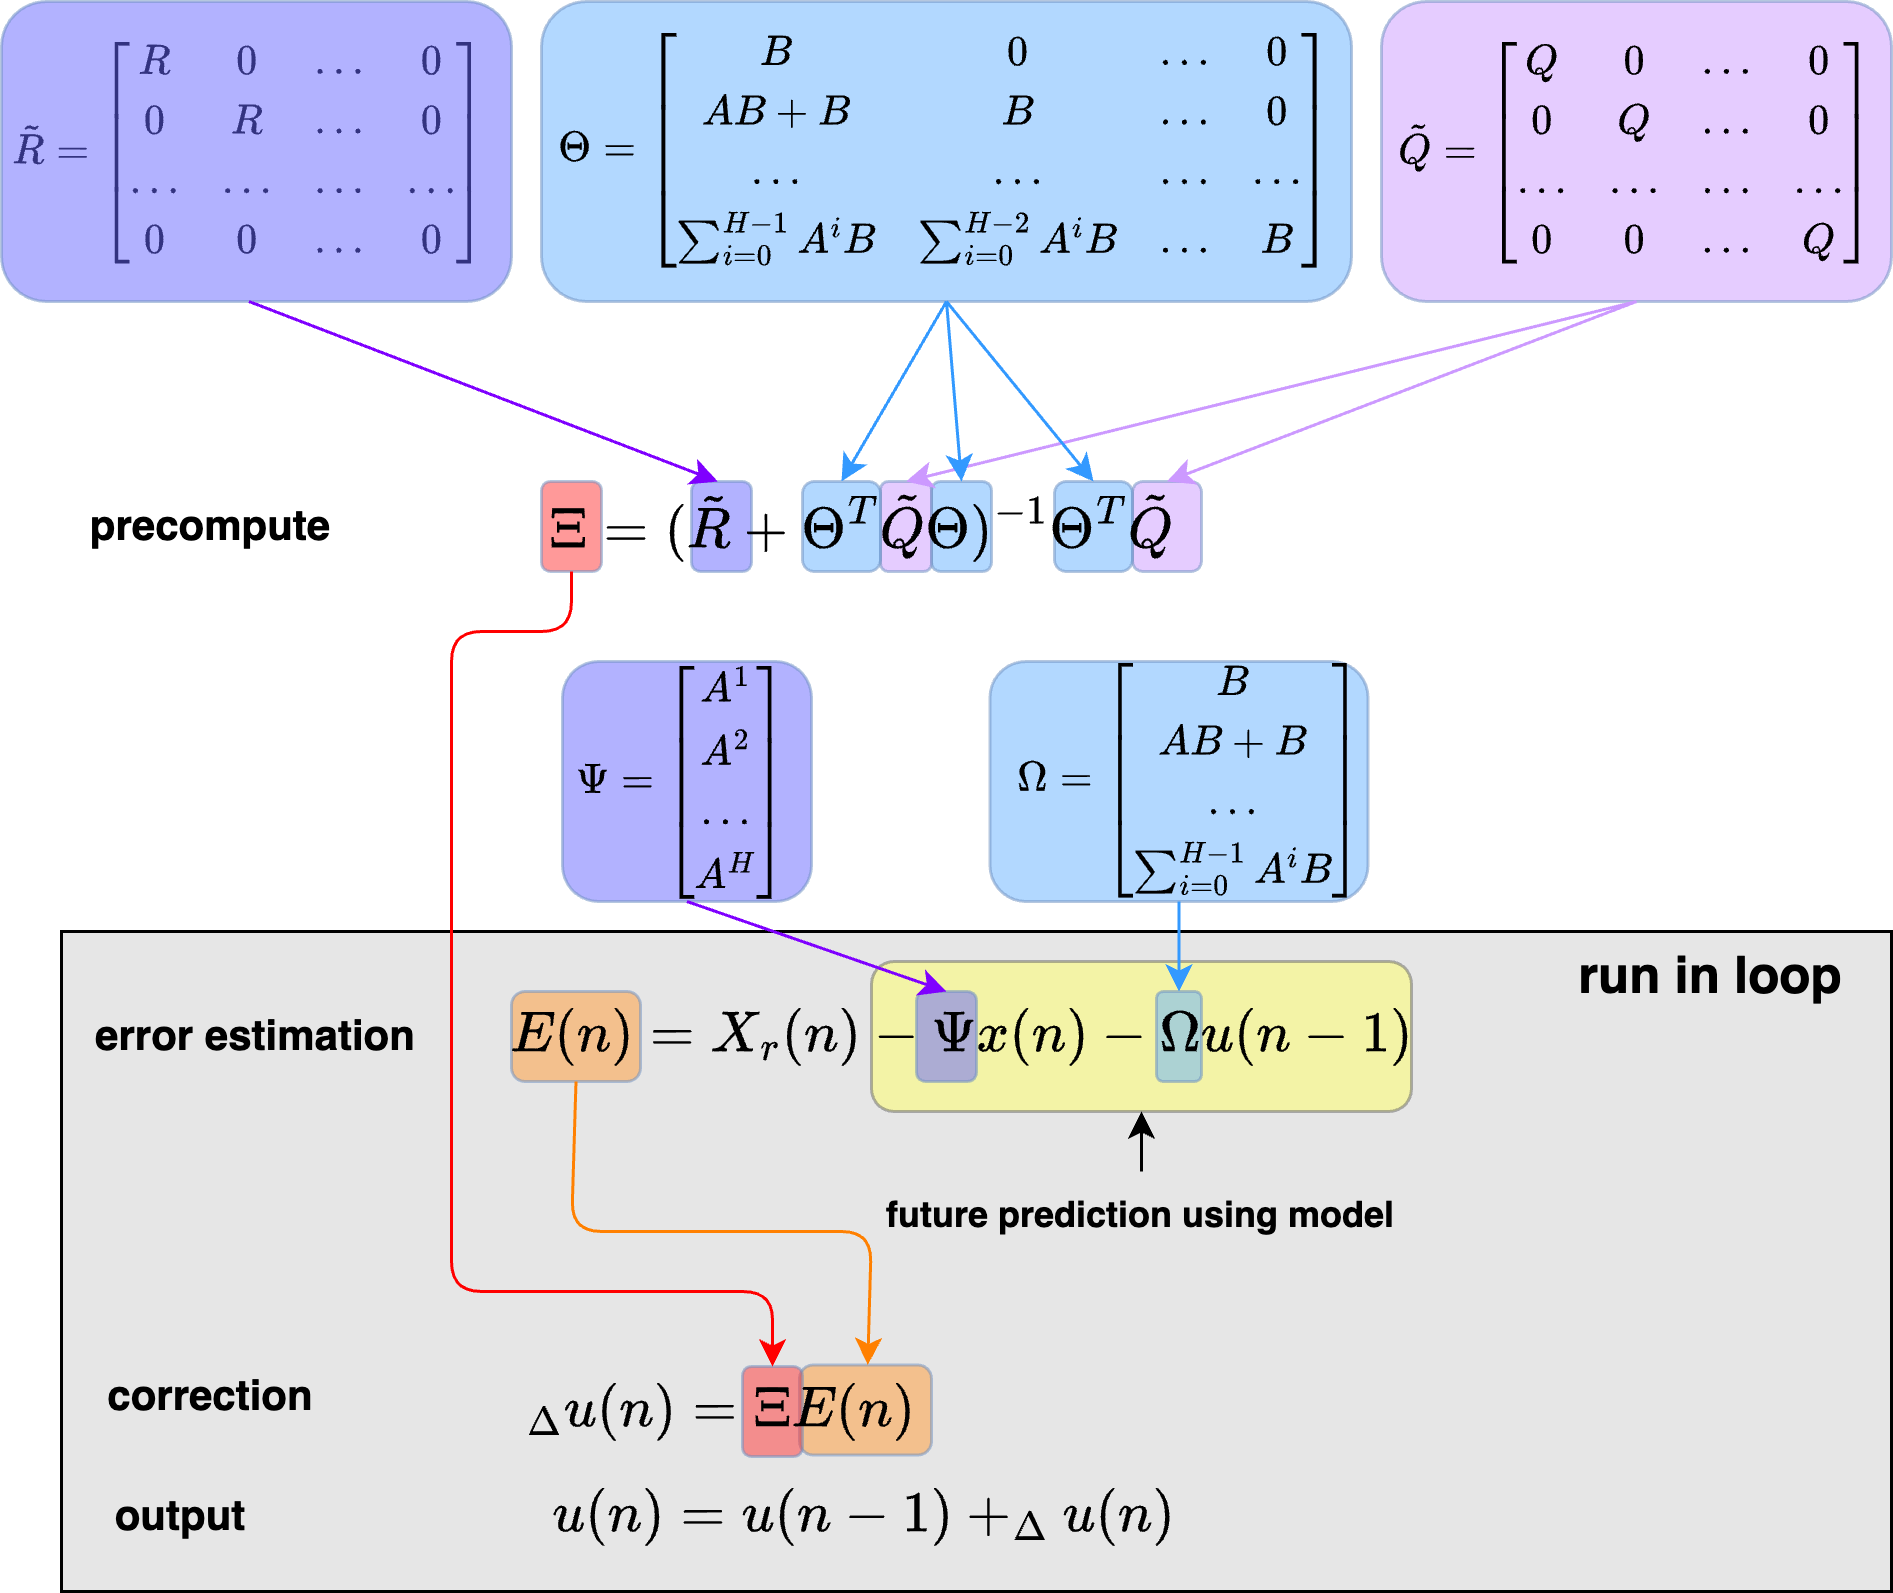
\includegraphics[scale=0.6]{../diagrams/control/control-mpc_algo.png}}

\end{frame}


\begin{frame}
  
  \frametitle{\bf full algorithm}
  given matrices : $$\tilde{Q}, \tilde{R}, \Psi, \Omega, \Theta$$
  initialization (precompute) :
  \begin{align*}
  \Xi &= (\tilde{R} + \Theta^T\tilde{Q}\Theta)^{-1} \Theta^T\tilde{Q} \\
  \end{align*}
  
  in loop :
  \begin{align*}
    E(n) &= X_r(n) - \Psi x(n) - \Omega u(n-1) \\
    _\Delta u(n) &= \Xi E(n) \\
    u(n) &= u(n-1) + _\Delta u(n)
  \end{align*}
\end{frame}




\begin{frame}
  
  \frametitle{\bf full algorithm - optimisation}
  \centering{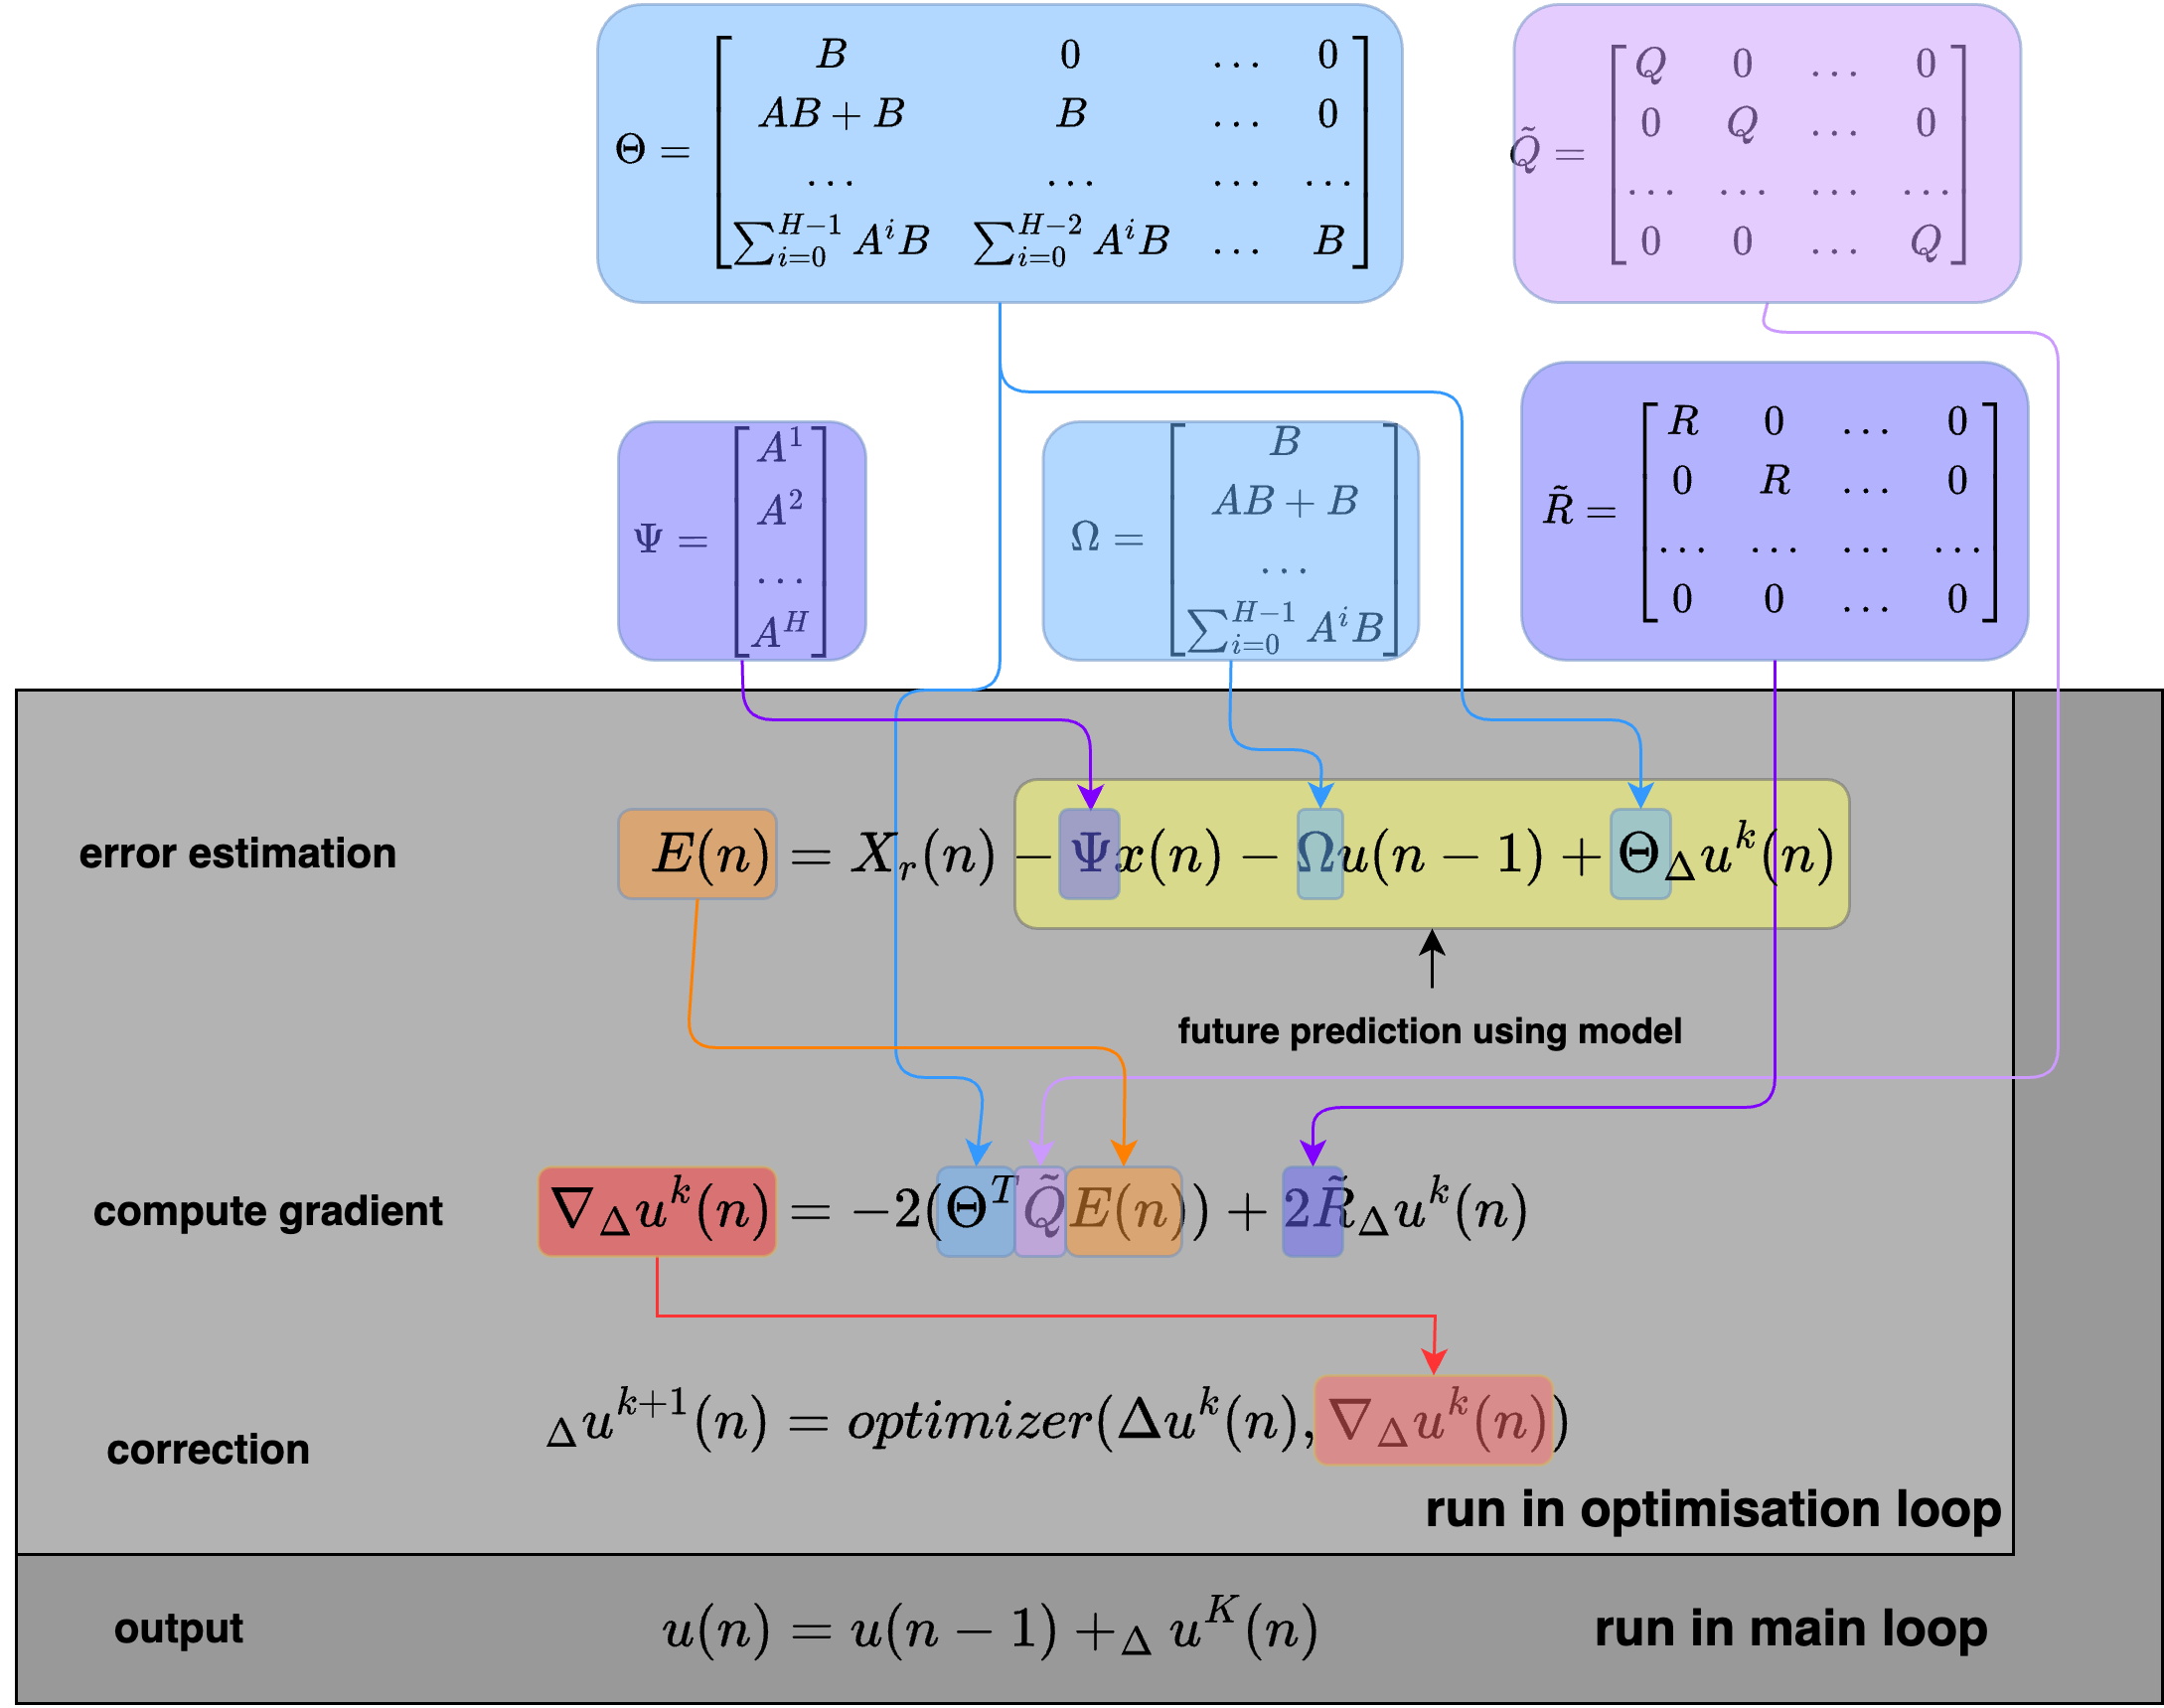
\includegraphics[scale=0.57]{../diagrams/control/control-mpc_opt_algo.png}}

\end{frame}



\begin{frame}
  
  \frametitle{\bf handling constrains}

  most common cliping ranges: 
 
  \begin{align*}
    _\Delta\tilde{u}(n) &= clip(_{\Delta}u(n), _\Delta u_{min}, _\Delta u_{max}) \\
    u(n) &= clip(u(n-1) + _\Delta\tilde{u}(n), u_{min}, u_{max})
  \end{align*}

  keep $u_{\omega}$ maximum possible and find constrains for $u_v$
  \begin{align*}
    v_{max} &= 2\pi R_{wheel}\frac{rpm_{max}}{60} \\
    v_{upper} &= min(v_{max}, -0.5Lu_{omega} + v_{max}) \\
    v_{lower} &= max(-v_{max}, -0.5Lu_{omega} - v_{max}) \\
    \tilde{u_v} &= clip(u_v, v_{lower}, v_{upper})
  \end{align*}
 

\end{frame}












\begin{frame}
  
  \frametitle{\textbf { recommended reading}}


  \begin{columns}

    \begin{column}{0.5\textwidth}
      \centering{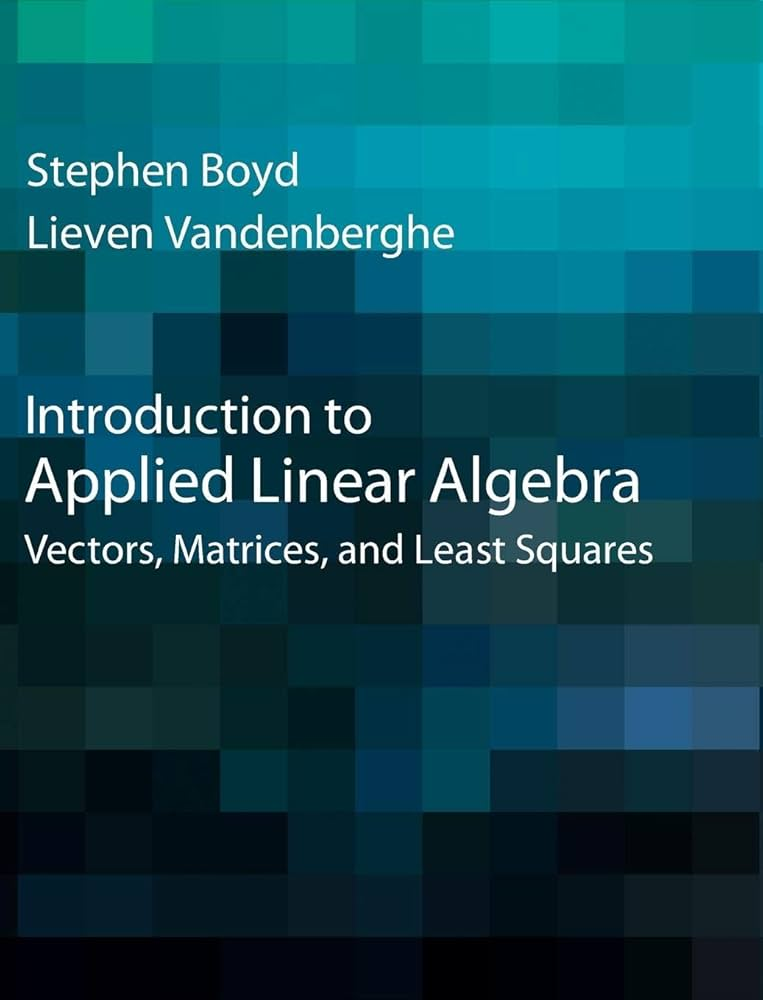
\includegraphics[scale=0.1]{../images/books/lin_alg.jpg}} \\
      \centering{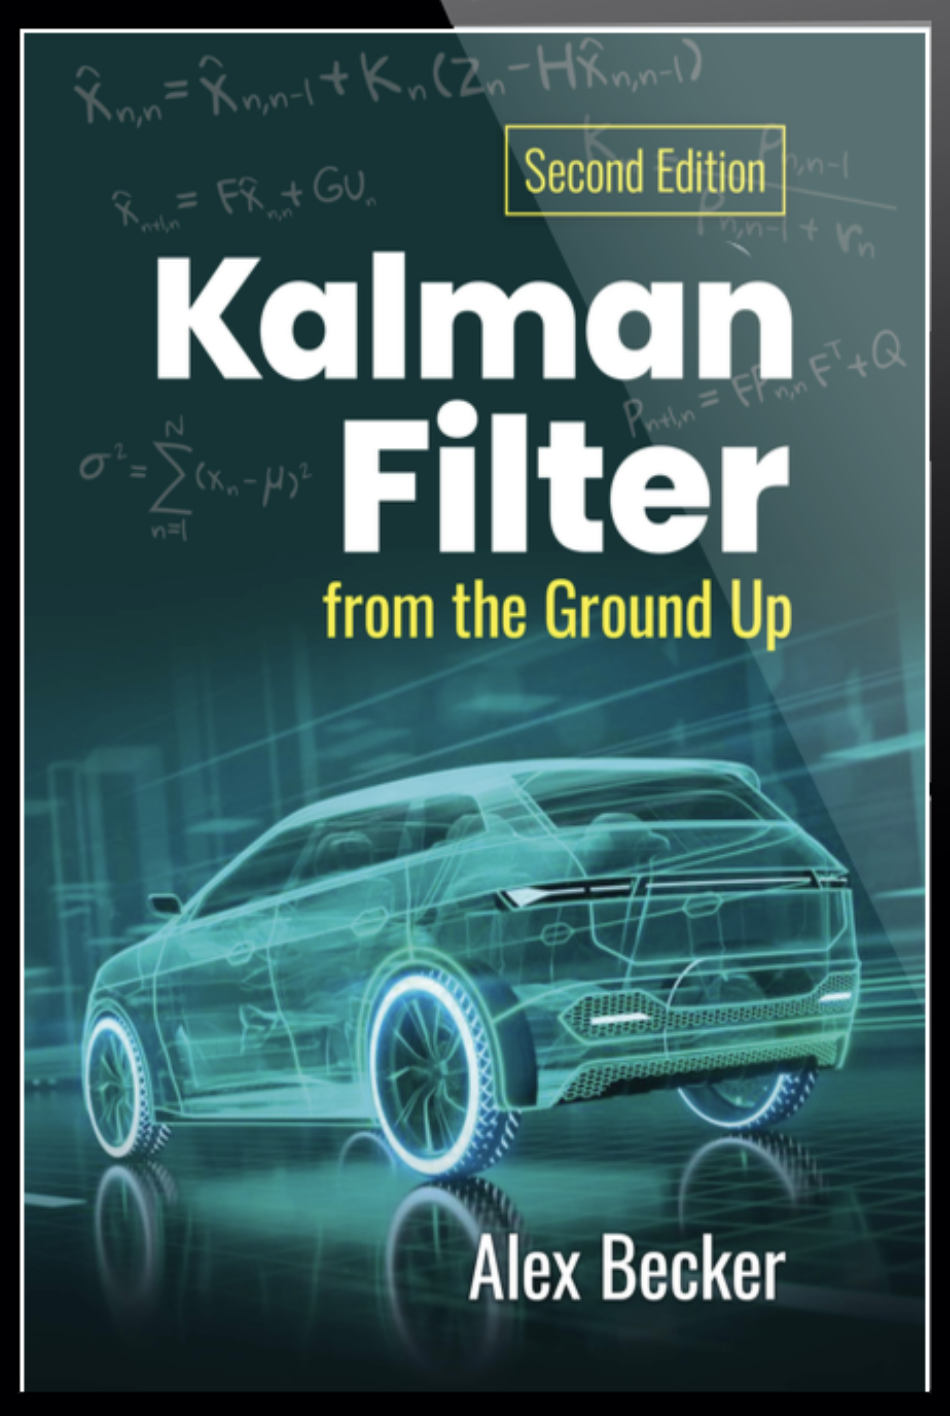
\includegraphics[scale=0.15]{../images/books/kalman_filter.png}}
    \end{column}

    \begin{column}{0.5\textwidth}
      \centering{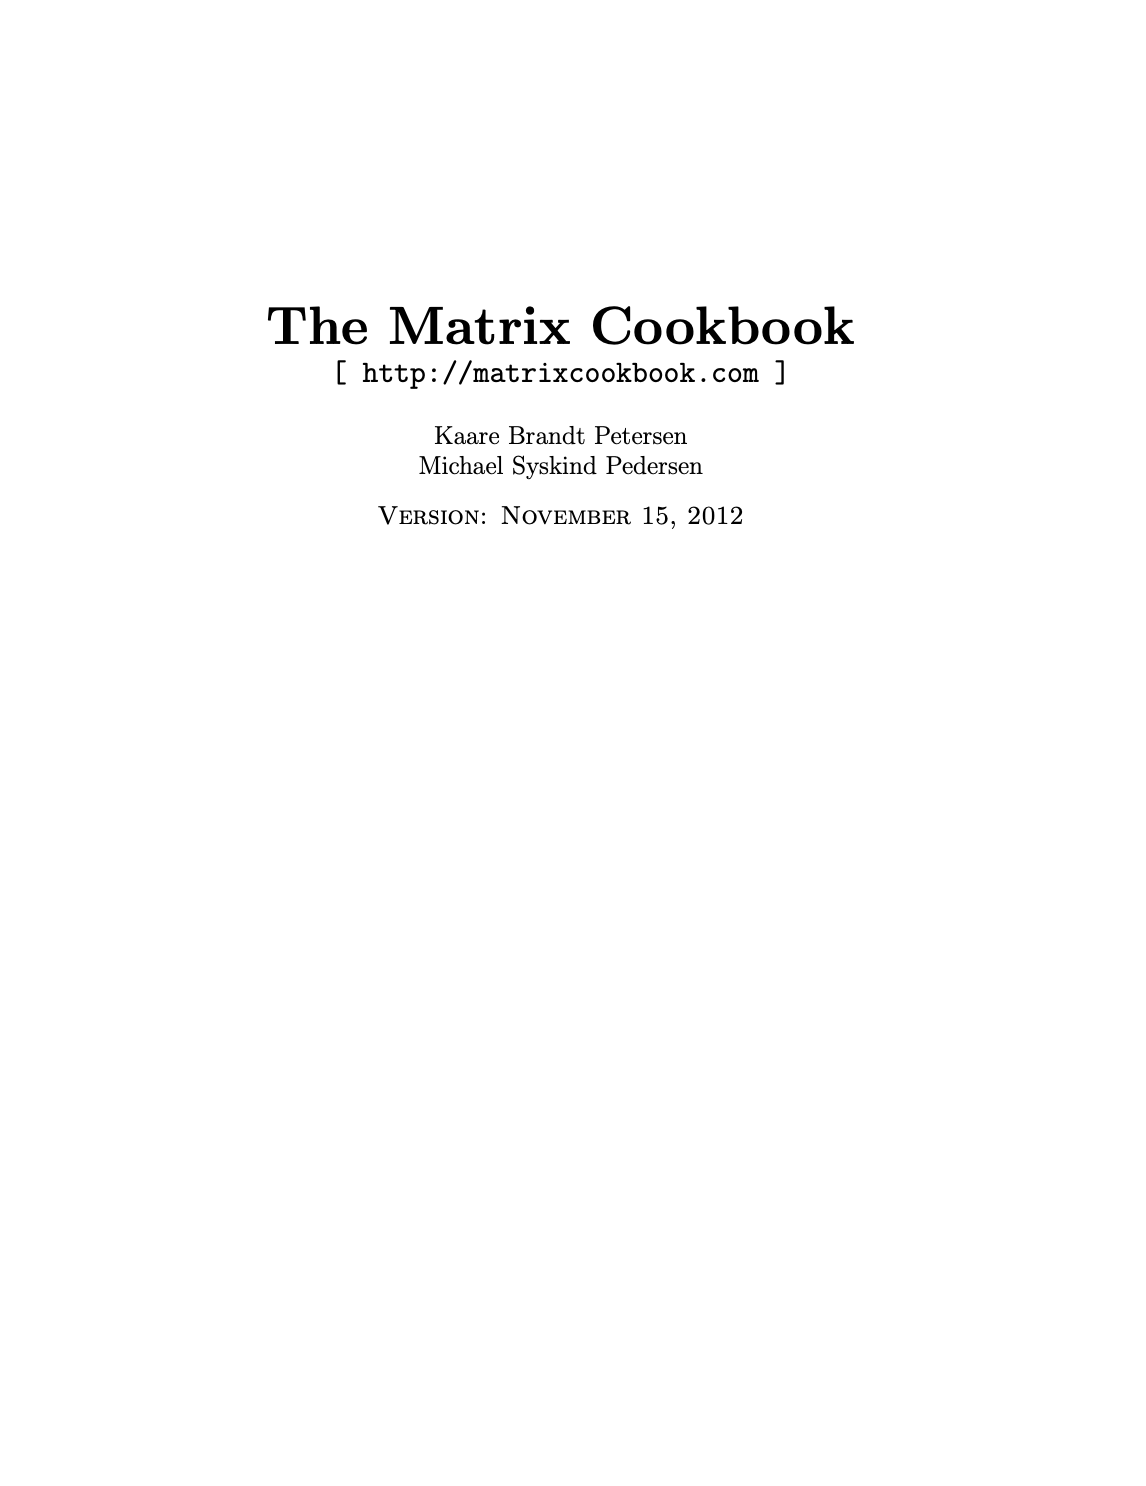
\includegraphics[scale=0.15]{../images/books/matrix.png}} \\
      \centering{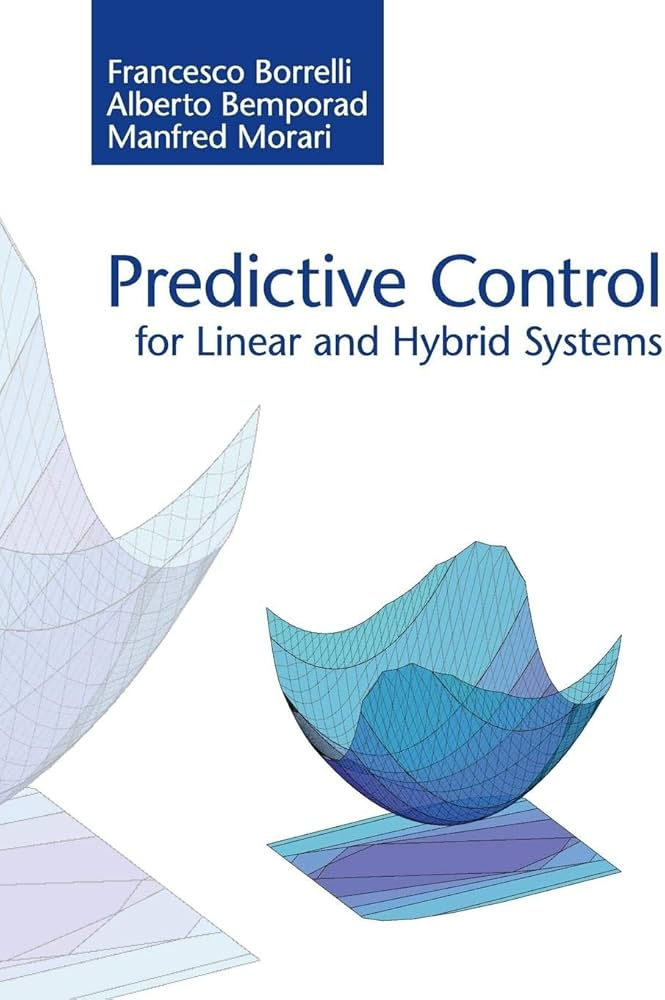
\includegraphics[scale=0.1]{../images/books/predictive_control.jpg}}
    \end{column}

  \end{columns}

\end{frame}



\end{document}